\documentclass[longbibliography,nofootinbib]{revtex4-1}

\newcommand{\kms}{NuCypher}

\usepackage{listings}
\usepackage{graphicx}
\usepackage{amsmath}
\usepackage{subcaption}
\usepackage[labelformat=parens,labelsep=quad, skip=3pt]{caption}
\usepackage[margin=5pt]{subfig}
\usepackage[usenames]{color}

\usepackage{natbib}
\bibliographystyle{unsrtnat}

\renewcommand{\baselinestretch}{1.4}
\setlength{\parskip}{1em}
\definecolor{darkgreen}{rgb}{0.00,0.50,0.25}
\definecolor{darkblue}{rgb}{0.00,0.00,0.67}
\newcommand{\figref}[1]{Fig.~\ref{#1}}
\usepackage[breaklinks,pdftitle={NuCypher Network: Staking Protocol \& Economics}, pdfauthor={Michael Egorov, MacLane Wilkison, Arjun Hassard},colorlinks,urlcolor=blue,citecolor=darkgreen,linkcolor=darkblue]{hyperref}
\graphicspath{{pdf/}}

\usepackage[T1]{fontenc}
\usepackage{lmodern}
\lstset{
    basicstyle=\ttfamily,
    basewidth={0.5em, 0.5em},
    columns=fullflexible,
}

\begin{document}

\title{NuCypher Network: Staking Protocol \& Economics}

\author{Michael Egorov}
\email{michael@nucypher.com}
\author{MacLane Wilkison}
\email{maclane@nucypher.com}
\author{Arjun Hassard}
\email{arjun@nucypher.com}
\affiliation{NuCypher}

\begin{abstract}
This paper describes the protocol mechanisms designed to incentivize and sustain reliable service provision in the NuCypher network, including the regular distribution of a subsidy to actively staking service-providers. The subsidy is generated through the scheduled expansion of the native token's circulating supply, following a `two-phase' model designed to maximize service quality, operational efficiency and network decentralization. The paper covers the rules for stake management, including locking, splitting, extending and unwinding stakes, and explains the relationship between discretionary stake configurations and subsidy size; with particular focus on the extra incentive to commit to longer staking durations. The impact of individual configurations on global supply dynamics is deduced. Finally, an analysis of historical service-provider behavior in existing staking networks provides an empirical context for design and parameter choices.
\end{abstract}

\date{\today}
\maketitle

\section{Motivation \& Context}

The Nucypher network is an example of a \textit{decentralized service marketplace}, providing infrastructural services to digital applications/systems (`users') via a distributed array of independent node operators (`service-providers'), who run the same software but have discretion over certain service parameters. NuCypher's primary offerings, secrets management and dynamic access control, are a breed of scalable, privacy-preserving, censorship-resistant services – the strength of these three value propositions depending, to some extent, on long-term commitment to the network by a large, diversified population of service-providers. Additionally, aspects of NuCypher services necessitate concurrent work by multiple service-providers in order to be maximally secure and redundant.
\\\\
Hence, like many decentralized service marketplaces, and indeed centralized marketplaces, an abundance of reliable, committed service-providers is critical – and that the network establishes this state prior to the emergence of user adoption, lest the adoption be short-lived. As with any network, operating a node incurs various overheads, upfront and ongoing, and denominated in fiat, cryptocurrency and time. Moreover, eligibility for service provision in the NuCypher network is contingent on the acquisition and time-locking of collateral (`staking'), which burdens the service-provider with ongoing risk and opportunity cost. NuCypher users, who require the collateral of those serving them to remain locked for at least as long as their commercial engagement with the network – engagements which in some cases will last for months or years – protract this burden.
\\\\
If demand for NuCypher services rises sufficiently, direct payments from users (`fees') will sustain the operations of service-providers. However, before demand reaches this threshold, another stream of revenue is required – to incentivize a sufficient number of service-providers to join the network, and to subsidize the cost of their operations until a mature fee market materializes. Thus, a vitally important mechanism in the NuCypher protocol is the predictable distribution of subsidies to actively staking service-providers, realized through the growth of the native token's circulating supply. 
\\\\
The NuCypher protocol's \textit{monetary policy} – the design choices and parameters that govern this subsidy mechanism – is the primary focus of this paper. 

\section{Two-phase Subsidy Model}

\subsection{Overview}

\subsubsection{Basic Properties}
From the moment the NuCypher network launches, the protocol will begin minting new tokens and distributing them exclusively to actively staking service-providers. Token allocations will be proportional to the relative size of the stake\footnote{The share of user requests (`work') delivered to service-providers, and therefore exposure to fee-earning opportunities, is also proportional to the relative size of a service-provider's stake.}. Service-providers will be incentivized to commit to longer spans of service provision through a commensurate subsidy size, and to increase their stake size with the subsidies they receive (`re-staking'). The genesis supply – the number of tokens circulating at network launch – will be 1 billion tokens. Over the course of the network's lifetime – as $t$ approaches $\infty$ – the circulating supply will approach a maximum of roughly 3.885 billion tokens.

\begin{figure}[h!]
    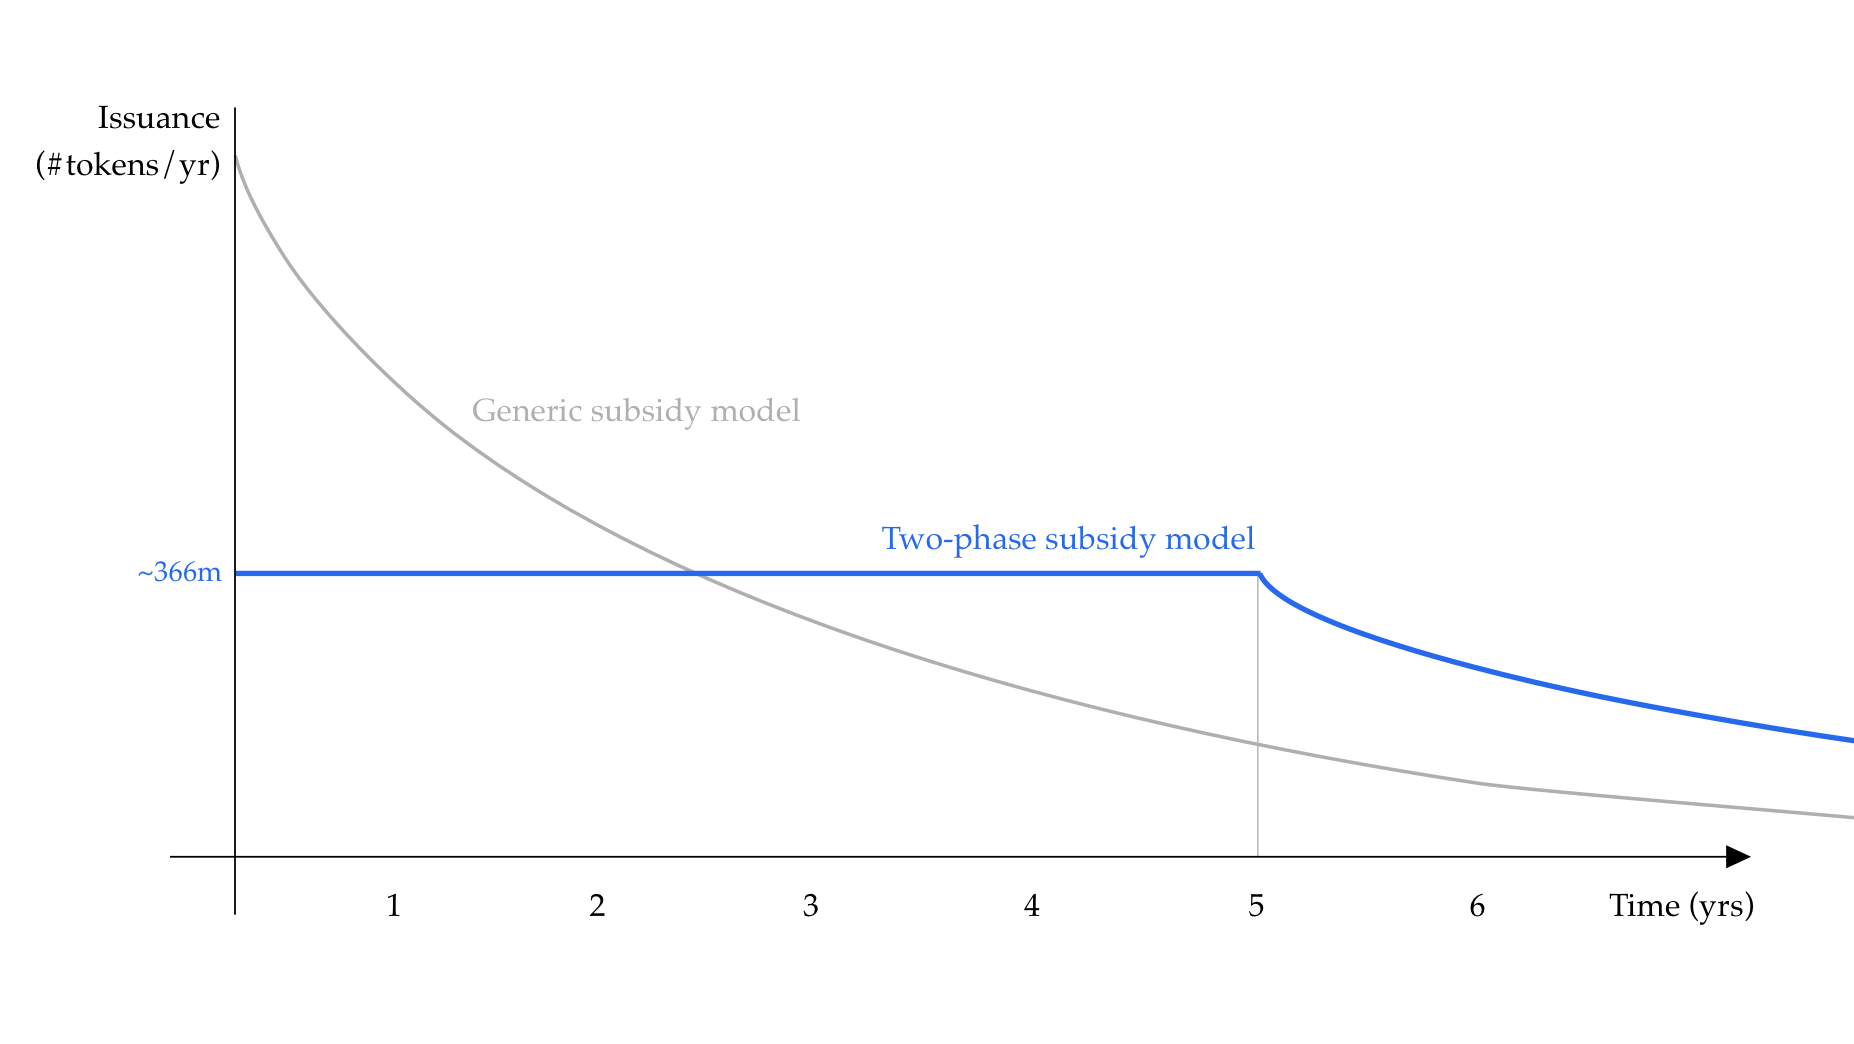
\includegraphics[width=0.8\textwidth]{Two_phase_model.png}
    \caption{Illustrative comparison of the two-phase subsidy model against a generic subsidy model. Note the y-axis refers to an absolute sum of tokens minted per year, as opposed to the growth rate of the supply (commonly referred to as the `inflation rate'). Both models see the supply growth rate decrease over time, but in the two-phase model, a phase of flat issuance implies a more gradual decline in the growth rate.}
    \label{fig:tp}
\end{figure}

\subsubsection{Phase 1 – Constant Issuance}
A prevailing characteristic of prominent decentralized networks is a subsidy that decreases over time; both in absolute terms (the total number of tokens distributed in a given period) and as a percentage of the circulating supply (the so-called `inflation rate')\footnote{The precise manner in which the subsidy decreases varies from network to network, including the periodic, irregular halving of block rewards, a smooth, exponential decline in the amount of tokens minted per day, and unscheduled, governance-driven subsidy reductions – the key commonality is that the number of tokens a service-provider is eligible to receive falls over time \cite{Decreasing-subsidy}.}. The NuCypher protocol diverges from this approach, enforcing a more \textit{temporally equitable} model, in which the maximum subsidy a service-provider can receive remains a constant, for at least the first five years of the network's existence. In this initial phase (`Phase 1'), a maximum of 365,915,960 new tokens will be minted and distributed annually\footnote{In the NuCypher protocol, global issuance is modified by the stake lock-up durations chosen by stakers. For the sake of simplicity, this paper initially discusses and parametrizes a scenario in which all service-providers choose to lock their stakes for 12 months or longer, thus receiving the maximum subsidy. In reality, the average stake lock-up duration is likely to be lower, which implies lower issuance in both phases. Regardless, lock-up durations are chosen entirely at the service-provider's discretion, and hence they retain control the size of subsidy received. However, variable issuance has an impact on the global economy and the moment in which the protocol switches from Phase 1 to Phase 2. This is covered in section III (Staking Protocol).}, equivalent to expanding the circulating supply by a maximum of 1,002,509.479 tokens every period (days). 

\subsubsection{Phase 2 – Decaying Issuance}
Phase 2 commences as soon as the circulating supply reaches a total of 2,829,579,800 tokens. The earliest the protocol can enforce the phase switch is exactly 5 years, or 1825 periods, after network launch. In Phase 2, fewer tokens will be minted in each successive period, such that the daily minting figure decays exponentially with a minimum half-life of 2 years. For example, on the second day of Phase 2, the maximum issuance is approximately 1,000,607 new tokens.

\subsubsection{Note regarding the `inflation rate'}

It is common in the monetary policy of decentralized networks to refer to the growth rate of the circulating token supply as the `inflation rate'. This paper avoids this terminology, focusing instead on the subsidy size – the absolute sum of tokens minted per period, or the \textit{issuance}, as a shorthand. In the two-phase model, Phase 1 sees a constant issuance in each period, so the supply growth rate decreases period-to-period (and year-to-year) – but more gradually than in a model with a decreasing or halving issuance. In Phase 2, the issuance also begins decreasing, which accelerates the decline in the supply growth rate. Some stakes will also experience a decreasing growth rate period-to-period, but this is strongly dependent on discretionary stake configurations – see FIG. (4) and FIG. (5). 

\subsection{Rationale for two-phase model}

\subsubsection{Demand uncertainty \& fragility}\label{demand}

The following demand-related premises form the basis of the two-phase model: 
\begin{enumerate}
\item There is little certainty regarding the length of time that will elapse between the network's launch and the development of meaningful demand from users (developers, end-users \& others).
\item Early-stage demand tends to be particularly fragile. Early adopters do not have the testimonials of existing users as evidence of a reliable or valuable service. Moreover, a greater proportion of the user base will be trialling the network for the first time. Compared with long-term users of the network in later epochs, for whom the price of abandoning the service is high (disruption to end-users, migration and new integration costs, etc.), trial-stage users will be less tolerant of inadequacies. For example, a single instance in which too few service-providers are available to immediately fulfill a sharing policy's requirements, may be enough to lose that user.
\item Subsidy models involving a precipitous drop in issuance rest on the assumption that demand will grow in a corresponding fashion, filling the gap in service-provider revenue. If demand grows slower than the model expects, some node operations may be rendered unsustainable, potentially destabilizing the network.
\item There may be some adopters of the NuCypher network whose use case inflexibly requires long-lasting sharing policies. For example, a stake that unlocks in 365 days provides a form of economic security, ensuring the policy will be served for the next 12 months by the associated service-provider. To fulfil the needs of early (and later) adopters with long-lasting policies, the protocol must motivate the successive re-commitment to long stake lock-up durations by an sufficiently large population of service-providers. A diminished subsidy, in lieu of a mature fee market, may not be enough to incentivize this repeated and essential re-commitment. 
\end{enumerate}

\\\\
Hence, the two-phase model attempts to mitigate the risk of \textbf{fledgling demand for network services coinciding with a disincentivized, dwindling or transient} service-provider population. Note that these premises do not contain strong claims about when (or if) meaningful adoption of the network will occur. Instead, it is the acknowledgement of uncertainty with respect to a demand timeline that forms the core of the problem, and underpins the utility and advantage of a stable issuance phase as part of a two-phase minting schedule. 

\subsubsection{Impeding centralization}

The allocation of subsidies in proportion to stake size can precipitate an unwanted side-effect – large, deep-pocketed service-providers, not needing to convert subsidies into fiat to cover operational costs, steadily increase the size of their stake (relative to smaller operators) and eventually consolidate control of the token supply. The threat of effective centralization through consolidation is a concern for a number of prominent decentralized networks\footnote{At the time of writing (May 2020) the top 5 largest stakers in Cosmos, Tezos and Irisnet control approximately 31\% \cite{cosmos}, 27\% \cite{tezos} and 22\% \cite{irisnet} of the bonded tokens respectively.}. 
\\\\
A counter-balance against centralizing dynamics of this sort is the incentivization and enrollment of new service-providers, who commence staking in later epochs (i.e. not at network launch). If issuance is at its highest in the earliest days of the network, but falls rapidly, genesis service-providers are granted an significantly greater head-start over newer entrants. This relates to an underlying rationale for the \textit{work token} thesis; the expectation that would-be service-providers will purchase the network's native token in order to stake and earn revenue \cite{work-token}. With a token issuance that decays from genesis, later-joining service-providers are doubly disadvantaged – they must pay the market price to acquire tokens, plus they receive a diminished subsidy. 
\\\\
Therefore, a two-phase subsidy model is a form of economic assistance to any would-be service-provider who doesn't happen to stake right at network launch, but decides to do so at a later date. By addressing the temporal inequity of immediately decreasing issuance, we impede problematic centralization trends.

\subsubsection{Risks to operational feasibility and pricing}

The bigger the difference in real-world value between the subsidies of early epochs and those of late epochs, the greater the risk of various perverse outcomes pertaining to the operations and strategy of service-providers. In the era of generous subsidies, highly inefficient operations will not only survive, but may increase their control of the circulating supply – and therefore, their share of future work (i.e. the percentage of forthcoming user requests and fees). As subsidies decline in value, inefficient service-providers who are incapable of adapting to lower revenues may be forced to cease operations, reneging on existing commitments to users and undermining the reliability of the service. Another undesirable outcome relates to the service pricing – when the issuance is very high, service-providers may tactically offer an unsustainably cheap service in an attempt to capture market share, with the intention of raising prices in later epochs, once subsidies dry up. Any users (developers and their end-users) that have become reliant on the service, but are unable to afford the new price point, may see their application and business thrown into jeopardy. This prospect presents serious friction for would-be users planning an integration and justifying the associated upfront costs and technical dependency.
\\\\
It is worth noting that market prices for comparable services (e.g. key/secret management) tend to be low, on both a per-operation and subscription (per-month) basis \cite{Pricing:AWS}\cite{Pricing:GC}\cite{Pricing:MS}. Profitability is achievable through a high volume of operations and/or users, which is almost certainly a long-term endeavor. This business context aggravates the risks of fast-falling subsidies described in this section. 

\subsection{Parametrizing the Two-Phase Model}

\\\\
In order to parametrize the two-phase model, we select certain invariants, and derive the other parameters from those constraints. We fix the total number of tokens ever to be minted, $S(\infty)$ at approximately 3.885 billion, and the minimum half-life of the issuance decay in the second phase, $T_{1/2}$, at 2 years. The genesis supply ($S_0$) is 1 billion tokens. Note that some numerical figures in this section are rounded for readability.
\\\\
The most important parameter for the subsidy schedule is the maximum number of tokens minted per period during the first phase, which we describe as the `max issuance' ($I_{max}$). Using an axiom for $S(\infty)$, we can derive $I_{max}$. $S(\infty)$ is the sum of (1) the tokens circulating at genesis, (2) the tokens minted in Phase 1, and (3) the tokens minted in Phase 2. Note that we initially express $I_{max}$ as a percentage of the genesis supply per year, before converting it to an absolute number of tokens per period – see Equation 7.

\begin{equation}
    S(\infty) = S_0  +  S_0 \cdot \int_0^{5} I_{max}(t)\, dt  +  S_0 \cdot \int_0^{\infty} I(t)\, dt
\end{equation}
\\
Note that we use 5 years as a provisional duration for Phase 1 in order to calculate the maximum possible issuance. In practice, the issuance will be lower, and hence the switching of phases ($T_{1\rightarrow2}$) will likely occur at $t$ > 5 years – see Equation 12. Note also that the boundaries of the second integral are $0$ and $\infty$, rather than $5$ and $\infty$, because the issuance curve in Phase 2 is computed independently of Phase 1. In Phase 2, the decaying issuance at a time $t$ is a function of $I_{max}$, since it commences at this figure.
 
\begin{equation}
    I(t) = I_{max} \cdot 2^{-\frac{t}{T_{1/2}}}
\end{equation}
\begin{equation}
    3.885 \cdot S_0  = S_0 + S_0 \cdot \int_0^{5} I_{max}(t)\, dt + S_0 \cdot \int_0^{\infty} I_{max} \cdot 2^{-\frac{t}{T_{1/2}}} \, dt ,\\
\end{equation}
\begin{equation}
    3.885 = 1 + 5 \cdot  I_{max} + I_{max} \cdot \left[\frac{-2^{(1-\frac{t}{2})}}{\ln{2}}\right]_0^\infty .\\
\end{equation}

\begin{equation}
    2.885 = I_{max} \cdot (5 + \frac{2}{\ln{2}})
\end{equation}

\begin{equation}
   I_{max} = \frac{2.885}{7.885} = 0.366
\end{equation}
\\
We multiply by $S_0$ and convert $I_{max}$ into the absolute number of tokens minted per period.

\begin{equation}
    \label{eq:abs}
   \frac{I_{max} \cdot S_0}{365} = 1,002,509.479\:\:max\:new \:tokens \:per \:period
\end{equation}
\\
A maximum of 1,002,509.479 tokens are minted every period until there are 2,829,579,800 billion tokens in the circulating supply. At this point the protocol will switch to Phase 2, in which a further 1,055,810,282 tokens will be minted until t = $\infty$.

\section{Staking protocol}

\subsection{Subsidy size and commitment time}

\subsubsection{Sub-stakes}

In order to be eligible to answer user requests, earn fees, and receive subsidies, a service-provider must commit to servicing the network for some period of time by locking collateral (staking). Service-providers specify a stake unlocking time in the future $t_1$, where at time $t$ the minimum duration $t_1 - t$ may not be fewer than $D_{\min}$ = 30 periods, but may be any greater number of periods .
\\\\
The NuCypher protocol allows service-providers to partition their stake into sub-stakes, up to a maximum of 30. A sub-stake has a unique remaining duration $D$ – the number of periods until it unlocks and the tokens become freely withdrawable. The sub-stake size $\theta$ is the number of tokens locked. It is possible to extend (but not reduce) $D$ for a sub-stake, or split a sub-stake by extending $D$ for part of it. It is also possible to acquire more tokens and increase $\theta$ in any sub-stake. This mechanism enables more granular planning for future liquidity needs. 

\begin{figure}[h!]
 \centering
    \begin{minipage}{0.48\textwidth}
        \centering
        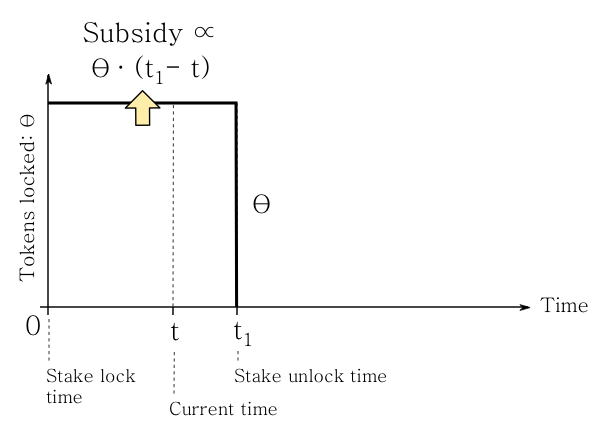
\includegraphics[width=0.99\textwidth]{graphs/one-step.png}
        \caption{A single stake which unlocks at time $t_1$. The stake receives a subsidy proportional to its size ($\theta$) and remaining duration to unlock ($D = t_1 - t$).}
    \end{minipage}\hfill
    \begin{minipage}{0.48\textwidth}
        \centering
        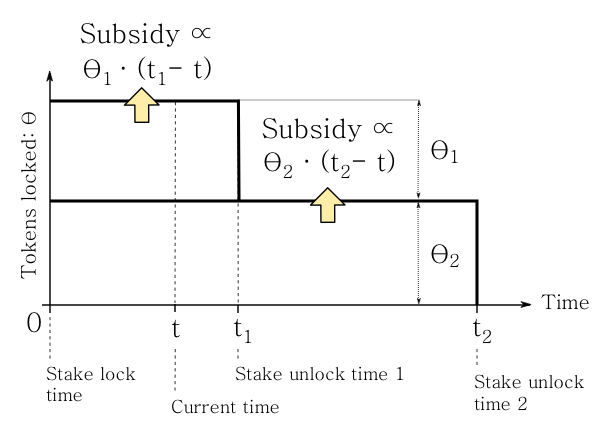
\includegraphics[width=0.99\textwidth]{graphs/two-steps.png}
        \caption{The stake in FIG. (3) has been split into two sub-stakes. This was achieved by extending the duration to unlock ($D_2 = t_2 - t$) for a portion (of size $\theta_2$) of the total tokens in the original stake. The two sub-stakes will receive differently sized subsidies.}
    \end{minipage}
\end{figure}

\subsubsection{Subsidy coefficient}

Secrets management and dynamic access control, the primary services offered through NuCypher, require service-providers to securely hold re-encryption keys and respond to access/revocation requests until the associated sharing policies expire. This involves maintaining a unique state on behalf of each user, which must persist without fail until the specified expiration – which in some use cases will not transpire for extended periods of time (12 months or longer). To ensure that service-providers stick around to perform these duties, the economic security of locked collateral must persist for at least as long as the sharing policies are active. Hence, the NuCypher protocol must further incentivize service-providers to lock their sub-stakes for as long as possible.
\\\\
As shown in figures 3 \& 4, the size of subsidy earned by each sub-stake $i$ is proportional to the duration of time until it unlocks ($D_i = t_i - t$), and the number of tokens in the sub-stake ($\theta$). Sub-stakes that unlock in 1 year or more receive the maximum subsidy ($\kappa=1$), whereas a sub-stake that unlocks in 1 month would receive slightly over half the maximum subsidy ($\kappa\approx0.54$). The subsidy coefficient $\kappa$ for a given sub-stake $i$ is calculated as following, where $D_{max}$ is currently set to 1 year or 365 periods:
\begin{equation}
    \kappa_i &=& \left(0.5 + 0.5 \cdot \frac{\min(D_i, D_{max})}{D_{max}}\right)
\end{equation}

In Phase 1, a sub-stake $i$ of size $\theta$ will receive the following subsidy, where $\Theta$ is the sum of all locked sub-stakes and $I_{max}$ is the maximum number of tokens that can be minted in a period $p$:

\begin{equation}
    \label{eq:ds}
    ds_{\theta i,p} = \kappa_i \cdot \frac{\theta_i}{\Theta} \cdot I_{max} 
\end{equation}

In Phase 2, a sub-stake $i$ of size $\theta$ will receive the following subsidy, where $S(\infty)$ is the total number of tokens ever to be minted (roughly 3.885 billion), $S_{p-1}$ is the circulating supply in the period before $p$, and $T_{1/2}$ is the issuance decay half life:

\begin{equation}
    \label{eq:rate-max}
    ds_{i,p} = \kappa_i \cdot \frac{\theta_i}{\Theta} \cdot \frac{\ln{2}}{T_{1/2} \cdot 365 } \cdot \left[S(\infty) - S(p-1) \right]\\
\end{equation}

\subsection{Variable issuance and the global economy}

The circulating supply at a given period $p$ is the sum of the tokens received thus far by all sub-stakes (this does not include the genesis supply):
\begin{equation}
    dS_p= \sum_i ds_{i,p}
\end{equation}

Sub-stakes locked for a short times earn less than the maximum subsidy, thereby slowing the expansion of the entire circulating supply – tokens are only minted if they are to be distributed to service-providers. The implication of any instance of $\kappa$ < 1 is that it will take longer than the provisional 5 years to mint all the tokens reserved for Phase 1. The year in which the protocol switches from the first to second phase ($T_{1\rightarrow2}$) is therefore: 

\begin{equation}
\label{phaseswitch}
    T_{1\rightarrow2}= \frac{S_{Ph1}}{S_0 \cdot \kappa^* \cdot I_{max}}
\end{equation}
\\
Where $\kappa^*$ is the average lock duration of all sub-stakes, weighted by relative size, and $S_{Ph1}$ is the total number of tokens reserved for Phase 1, excluding the genesis supply (roughly 1.83 billion). For example, if $\kappa^*$ were to equal 11 months, $T_{1\rightarrow2}$ would be 5 years and 79 days. The longest Phase 1 can last (i.e. if all sub-stakes unlock in 1 month, so $\kappa^* \approx 0.54$), barring changes to the protocol, is approximately 8 years and 209 days.

\subsection{Other considerations for service-providers}

\subsubsection{Re-staking}

A service-provider is free to withdraw the subsidies their sub-stakes receive. If they pocket all incoming tokens, then their sub-stakes will remain the same size, but are likely to decrease as a fraction of the total tokens staked ($\Theta$), which means their period-to-period subsidy, and exposure to user requests, will also decrease. A service-provider may re-stake their subsidies, provided they have the capacity to support the potential increase in workload (user requests). If the sub-stakes in question are set to unlock in 1 year or longer, and the average lock duration is shorter than this, then re-staking all subsidies would see those sub-stakes grow and account for a increasing fraction of the total tokens staked. As a result, the subsidies received would also rise over time. The dramatic difference in long-term cumulative earnings between various staking strategies over both phases is shown in FIG. (4) and FIG. (5). 

\subsubsection{Winding down sub-stakes}

The default setting for a sub-stake $i$ is for $D_i$, the duration of time until the unlock date, to be automatically prolonged. This holds the subsidy coefficient ($\kappa_i$) constant. If a service-provider proactively initiates a wind-down – that is, they specify an unchanging unlock date in the future, then the corresponding subsidy will continually decrease as the duration to unlock gets smaller and smaller, until $\kappa_i$ reaches a minimum of $0.5$.

\subsubsection{Staking rate}

The \textit{staking rate} is the percentage of tokens staked out of the total circulating supply in a given period. Other decentralized networks refer to this variable as the `participation rate' or `total staked'. Since subsidies are derived from expanding the token supply, which dilutes all holders of the token, the true value of a subsidy distributed in a given period is inversely proportional to the staking rate in that period. In other words, the fewer other stakers receive subsidies, the more they're worth. The calculations that produced the graphs in FIG. (4) and FIG. (5) assume a constant staking rate of 70\% over the 12 years shown.

\begin{figure}[h!]
    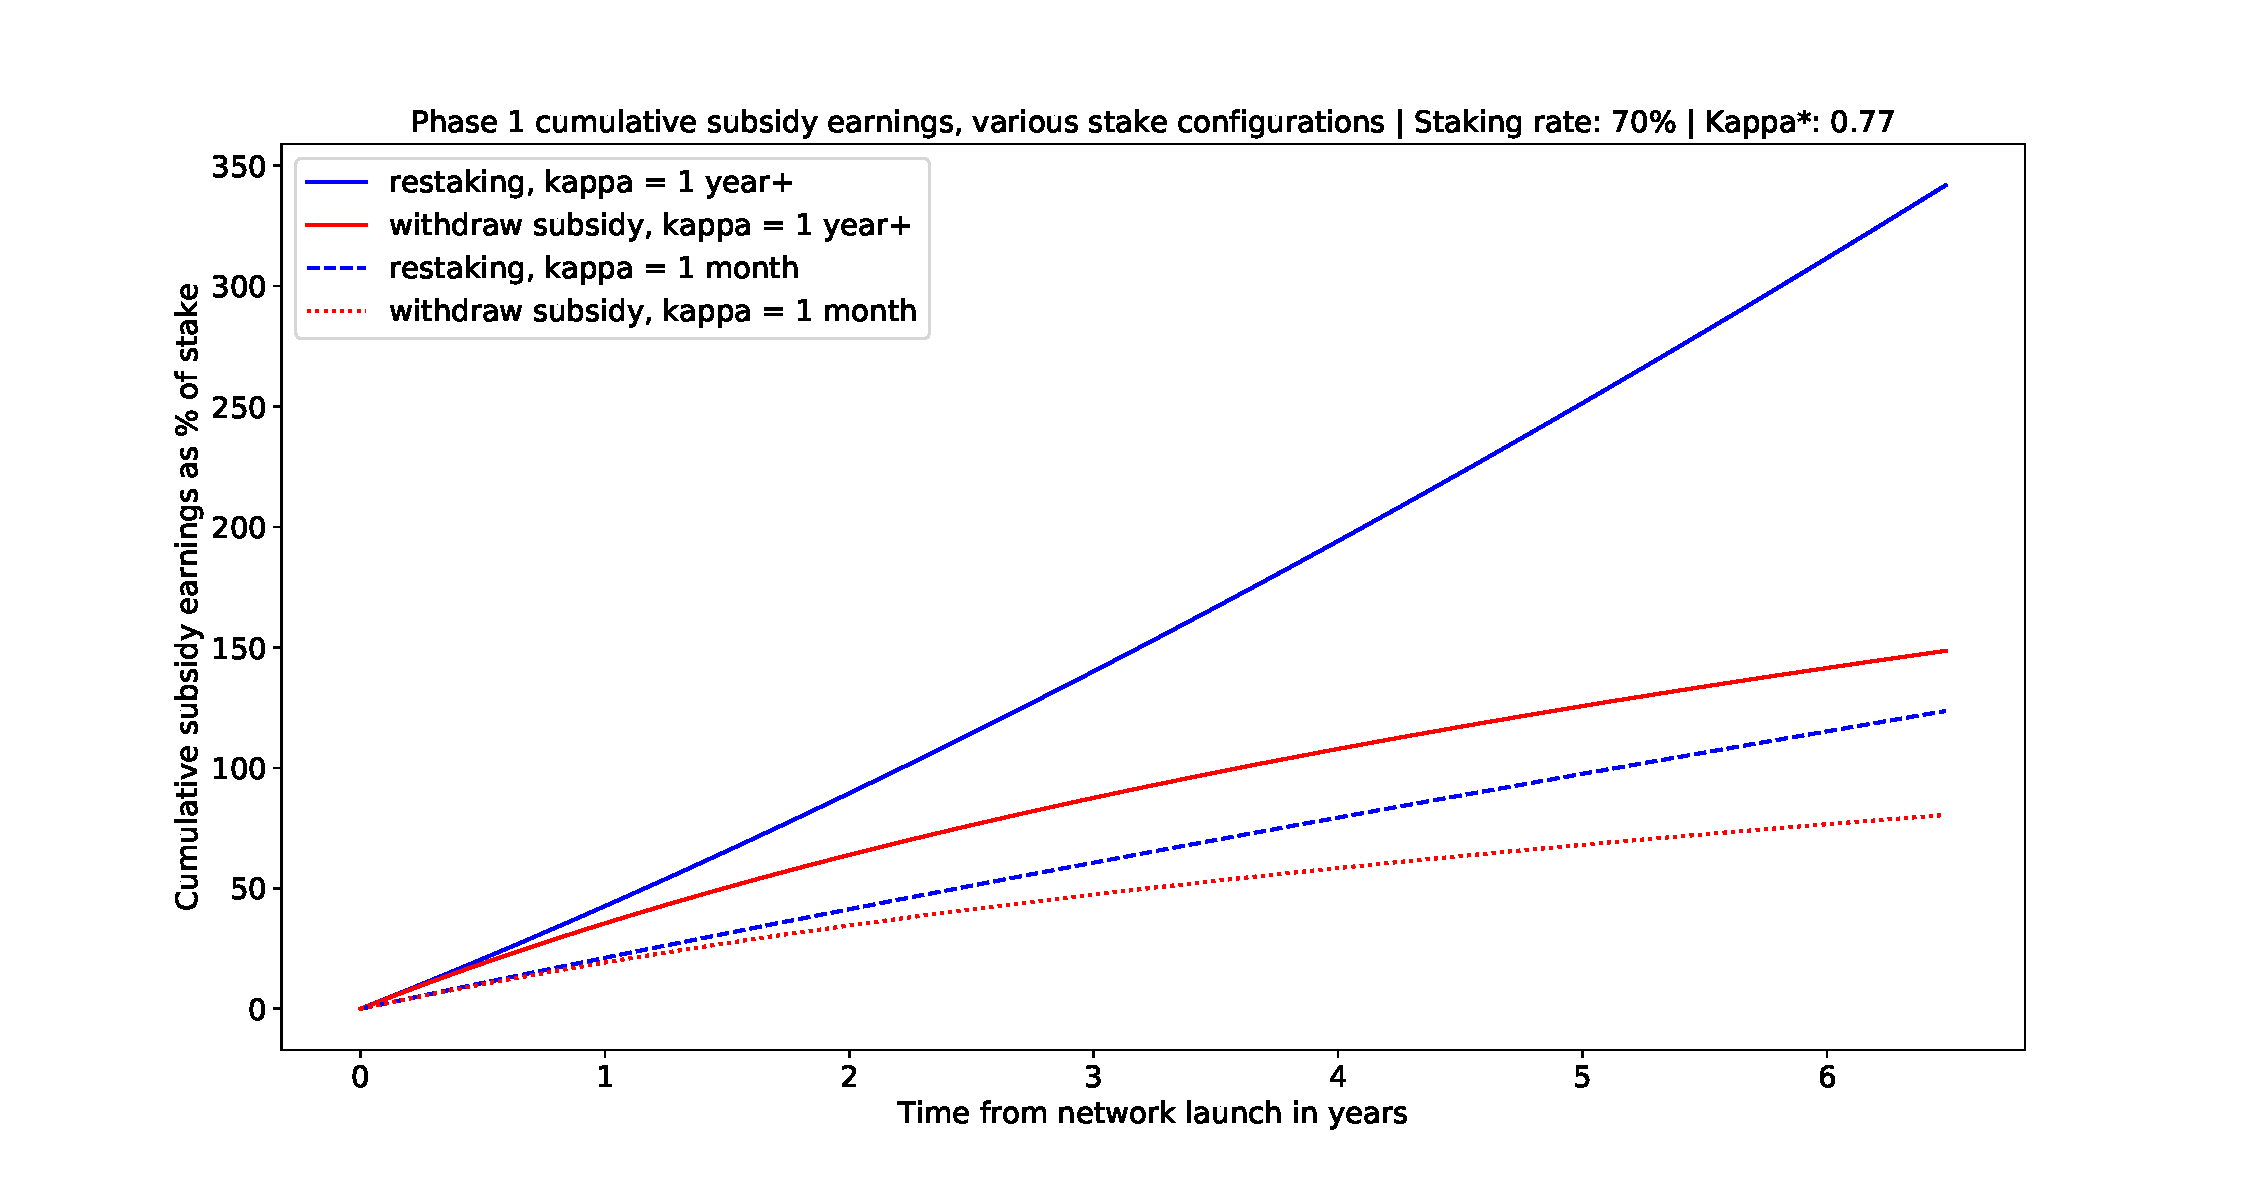
\includegraphics[width=\textwidth]{graphs/SubsidyP1.pdf}
    \caption{Cumulative total subsidies received in \textbf{Phase 1}, for stakes unlocking in 12+ and 1 month, and configured to re-stake or withdraw subsidies. Staking rate \& average lock duration assumed to be 70\% and 0.77 respectively.}
    \label{fig:tp}
\end{figure}

\begin{figure}[h!]
    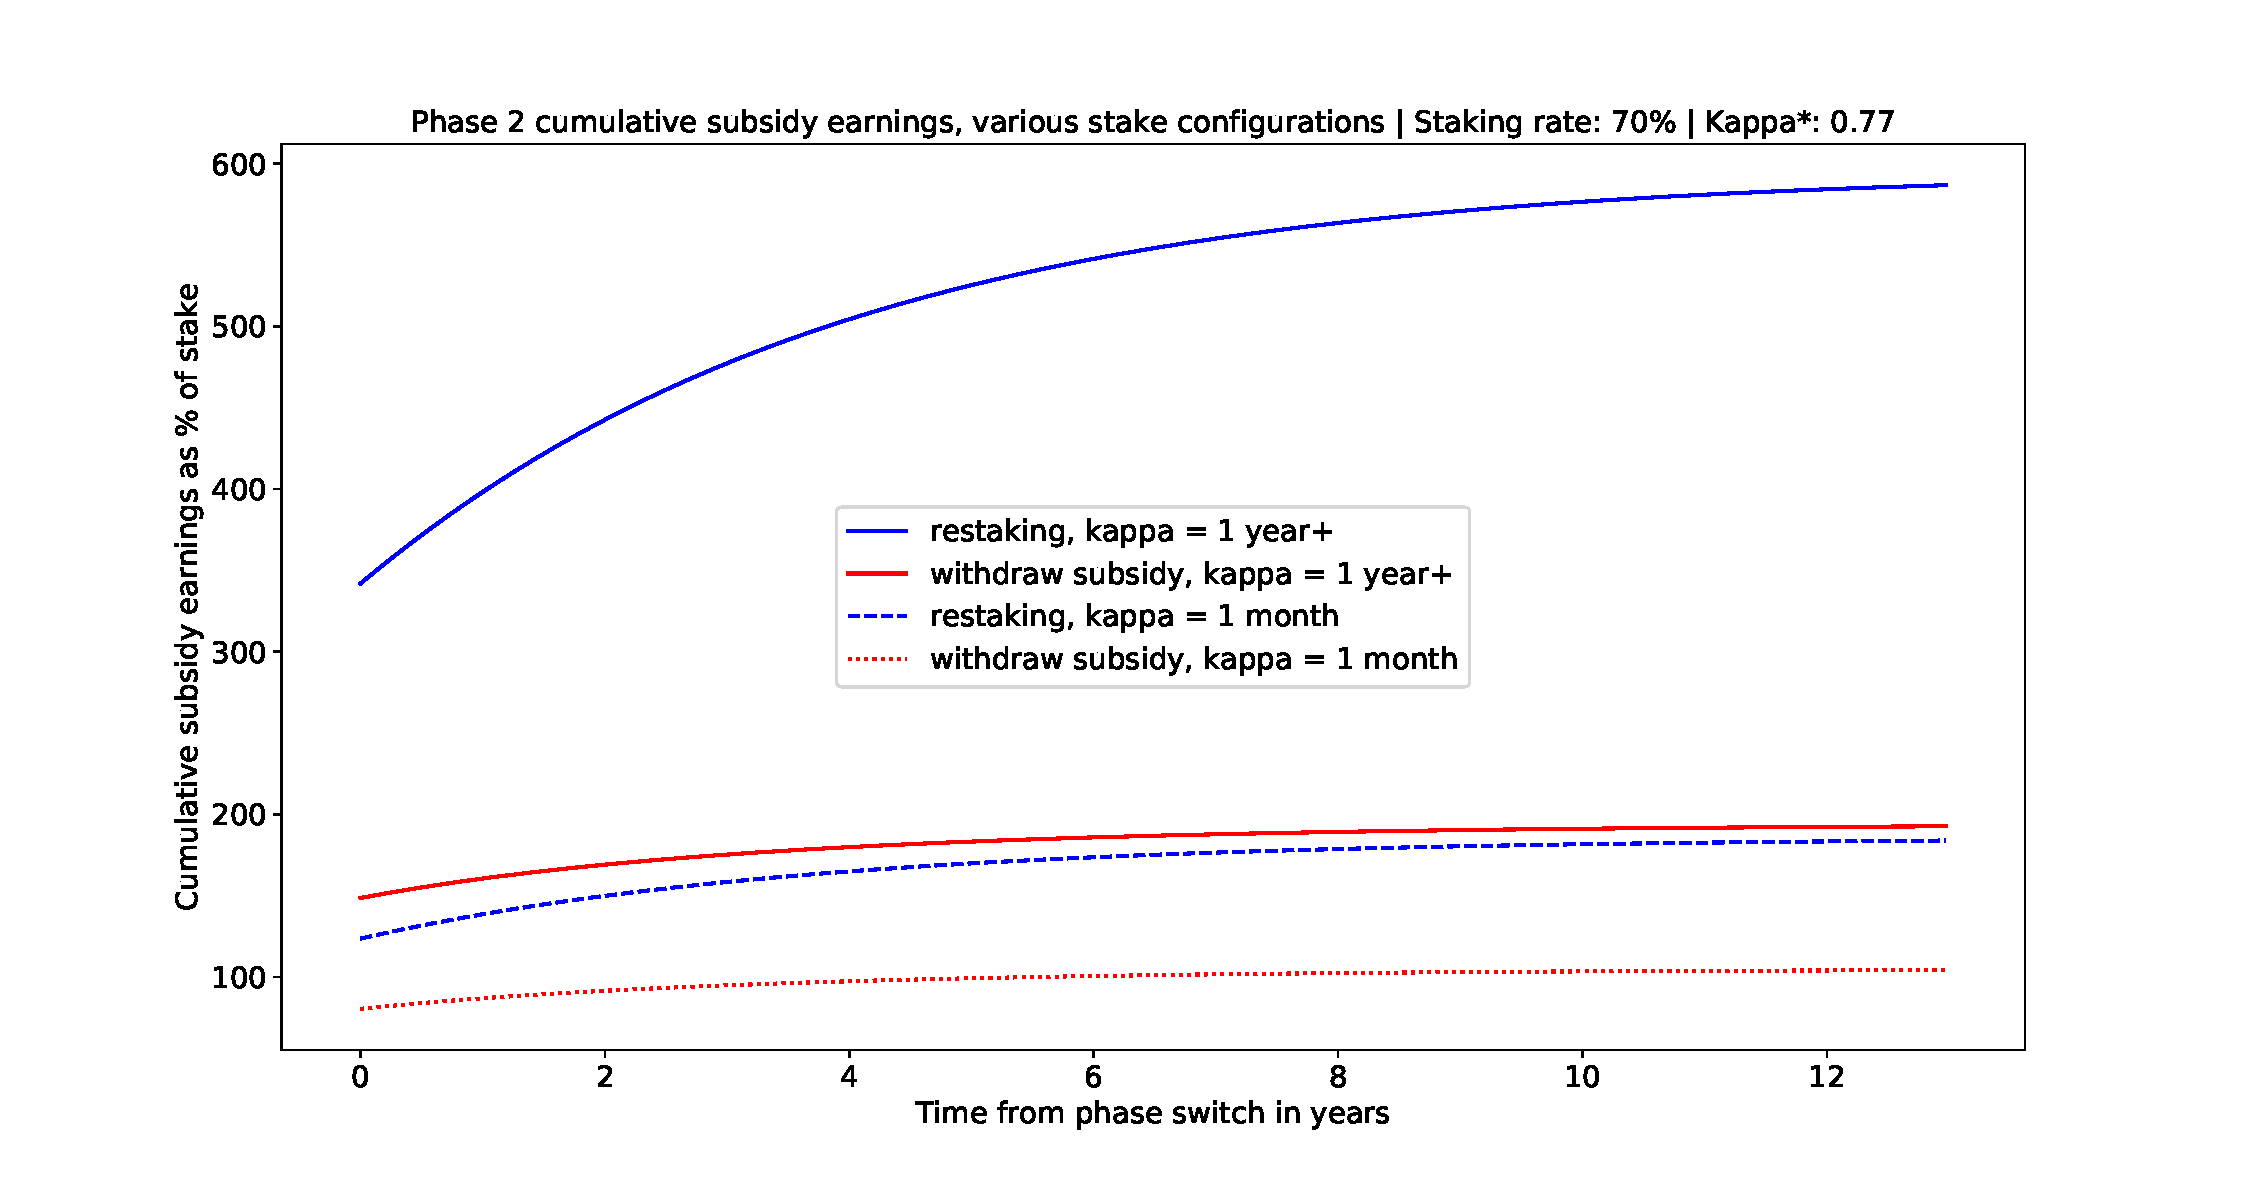
\includegraphics[width=\textwidth]{graphs/SubsidyP2.pdf}
    \caption{Cumulative total subsidies received in approx. first 7 years of \textbf{Phase 2}, with all other parameters the same as FIG. (4). Note that all totals at the end of Phase 1 equal those at the start of Phase 2.}
    \label{fig:tp}
\end{figure}

\section{Empirical analysis of existing networks}

\textit{Full study to be published. This section summarizes analysis thus far and evaluates results with respect to the two-phase model.}

\subsection{Outline}

\subsubsection{Objectives \& Data Characteristics}

The objective of this analysis is to better understand the relationship, if any, between (1) the variable real value of a subsidy received by service-providers/stakers accounting for the staking rate and dilution (the \textit{real yield}), and (2) their subsequent, collective decision to increase, decrease or maintain the size of their stake, expressed as a percentage of the total circulating tokens (the \textit{staking rate}). This pertains directly to the primary objective of the NuCypher staking protocol mentioned in section 1 – to maximise the abundance and reliability of network supply – which is reflected in the health\footnote{`Health' in this context simply refers to the percentage of tokens staked – for example, a network with only 5\% of tokens staked might be described as unhealthy, because it's likely to be more centralized, less secure, and lack the capacity to deal with demand.} and stability of the staking rate. This study employs data sets from two independent sources, (A) Staking Rewards and (B) Yields:
\\\\
(A) Staking Rewards provides data on the networks Tezos, Cosmos, Livepeer and Irisnet. The Staking Rewards time series is 4x daily (every 6 hours) and runs from February 2019 (Livepeer), March 2019 (Cosmos \& Irisnet) and July 2019 (Tezos) until February 2020 (all four networks). 
\\\\
(B) Yields provides data on the networks Tezos, Cosmos, and Livepeer. The Yields time series is daily and runs from July 2019 (Tezos \& Cosmos) and September 2019 (Livepeer) until April 2020 (all three networks).
\\\\
For the networks in both data sets, there are discrepancies between equivalent readings on overlapping days. This may be due to different methods of calculating both variables, but it is beyond the scope of this study to reconcile the data or decide which is superior, and so both sets of results should be interpreted with equal weight, or weighted by an objective factor like sample size or missing entries. It is worth mentioning that these data entries have been calculated and compiled by (A) professional data providers whose products depend on data accuracy, and (B) professional staking operators that currently stake in all the networks in question. Thus both data sets certainly reflect \textbf{an} authentic economic reality, if not \textbf{the} economic reality. 

\subsubsection{Relevant system dynamics}\label{dynamics}

In all the networks under examination, when the staking rate increases, the real yield decreases immediately by a similar magnitude, and vice versa. This is because the amount of stake eligible for a subsidy increases, but the total subsidy available at that same timestamp doesn't change (or changes a relatively small amount) - this means there are more stakers to split the same total subsidy. This is a known, causal relationship, that we expect to witness when the time lag between the variables is zero. 
\\\\
The networks have different rules for increasing and reducing the size of a stake (often referred to as `bonding' and `unbonding' respectively), but typically it is asymmetric – a staker may deposit tokens more rapidly than withdraw. Livepeer stakers must wait about 7 days after triggering a withdrawal, Tezos requires a 1-2 day wait, and Cosmos \& Irisnet require 21 days. The time it takes for stakers to respond to changes in the real yield is further affected by the significant proportion of tokens that are \textit{delegated} to professional stakers. In general, we assume that changes in the real yield are also experienced by delegators, and they react accordingly, if not in the same manner as stakers. A rigorous evaluation of the impact of bonding/unbonding asymmetry and delegator behavior on the relationship between the real yield and staking rate is left for future work.

\subsection{Results}

\subsubsection{Methodology}

The graphs in this section show the cross-correlation (Pearson) between the time series of the real yield and the time series of the staking rate, across a range of time-lags. Before the lagged cross-correlations were computed, all time series were \textit{detrended} by training a linear regression model on the data, then subtracting the resulting trend from the data. All time series were also \textit{differenced}. These two steps significantly reduce the autocorrelation and time-dependent structure of the data, granting the cross-correlations greater validity. Finally, all time series were `lumped' – using the 7, 14, 21 and 28 day mean to group the data. Each of these lump sizes – representing various degrees of data coarseness – are displayed and discussed individually.


\begin{figure}
 \centering
    \begin{minipage}{0.5\textwidth}
        \centering
        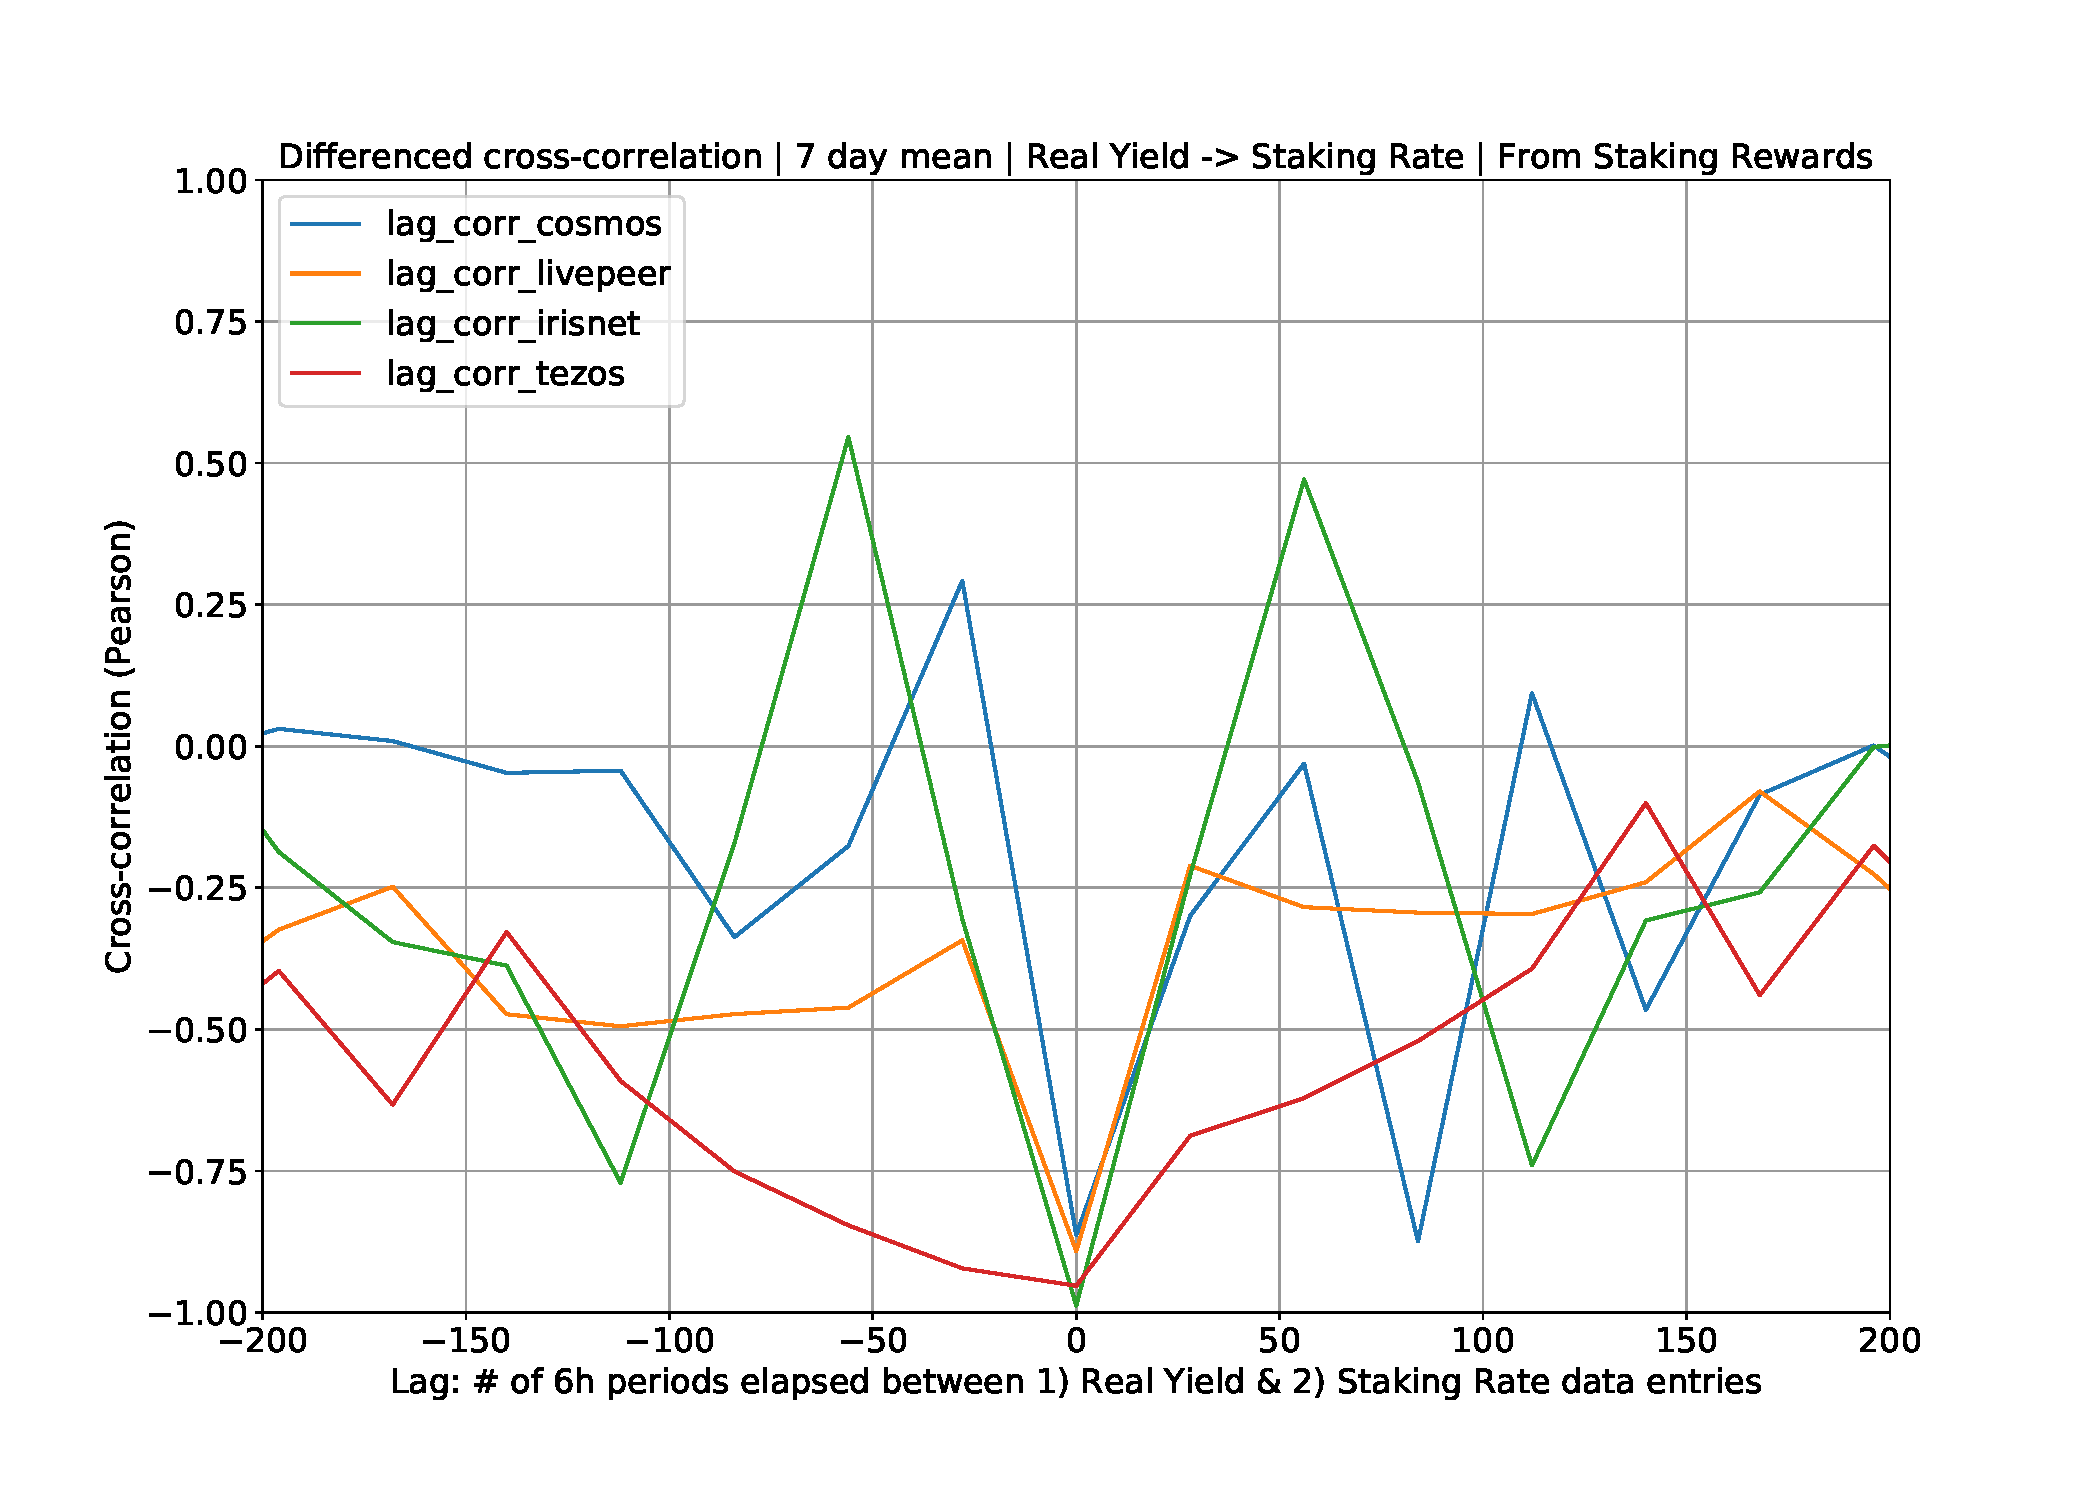
\includegraphics[width=1\textwidth]{graphs/CrossCorr_SR_DIF_7.pdf}
        \caption{7 day lump}
    \end{minipage}\hfill
    \begin{minipage}{0.5\textwidth}
        \centering
        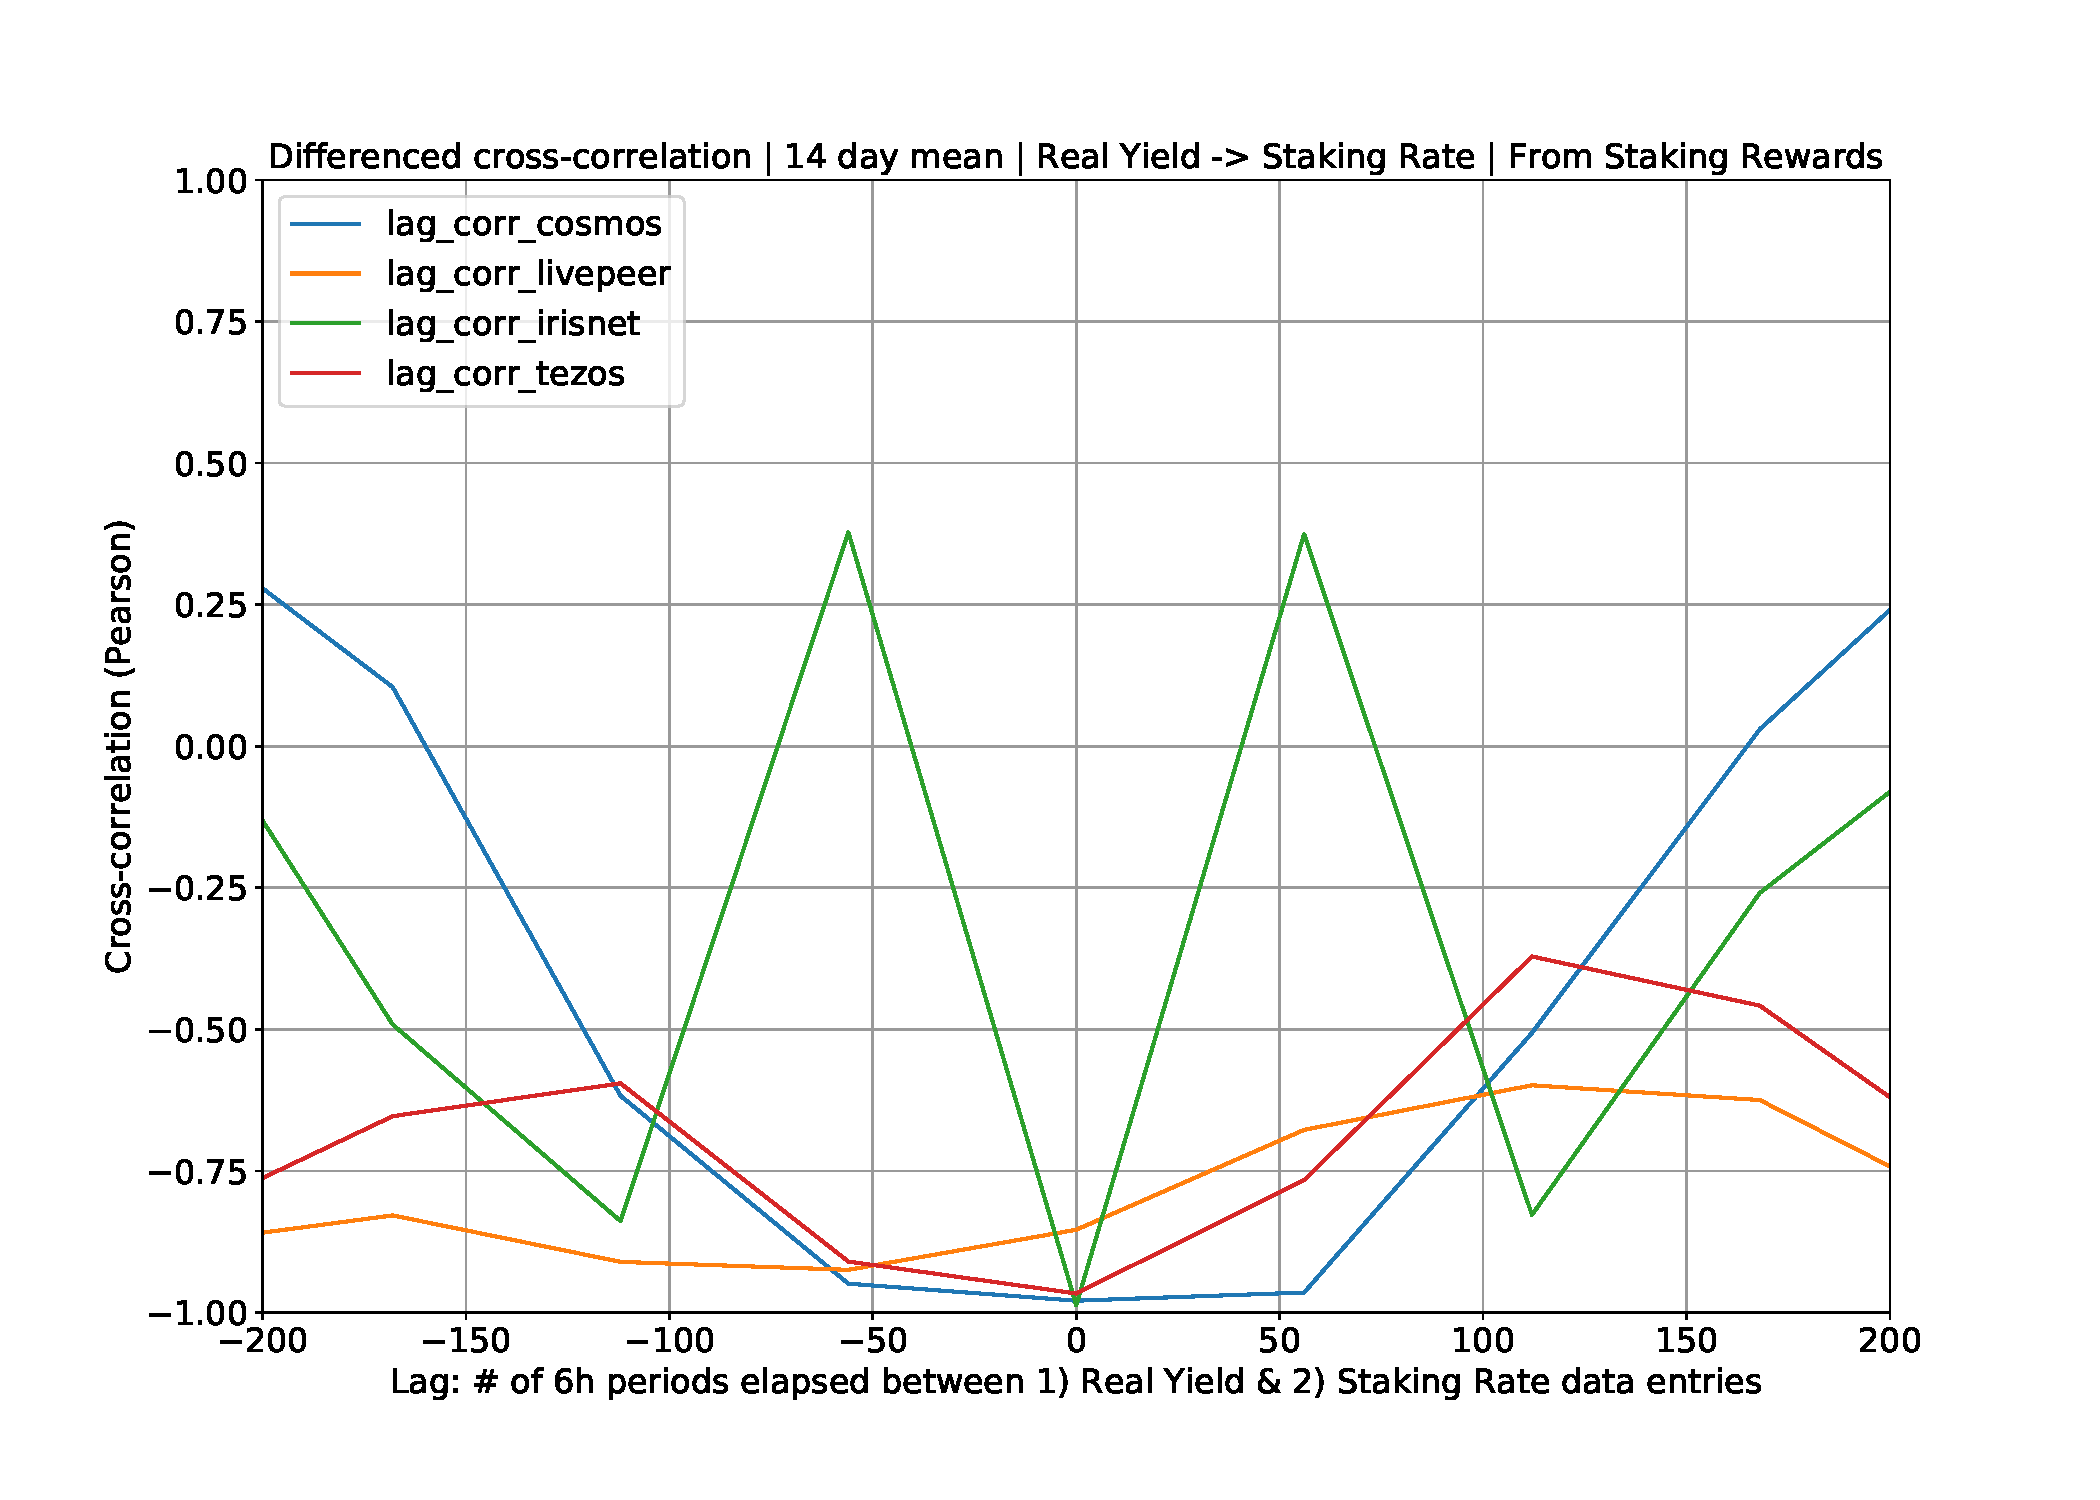
\includegraphics[width=1\textwidth]{graphs/CrossCorr_SR_DIF_14.pdf}
        \caption{14 day lump}
    \end{minipage}
    \begin{minipage}{0.5\textwidth}
        \centering
        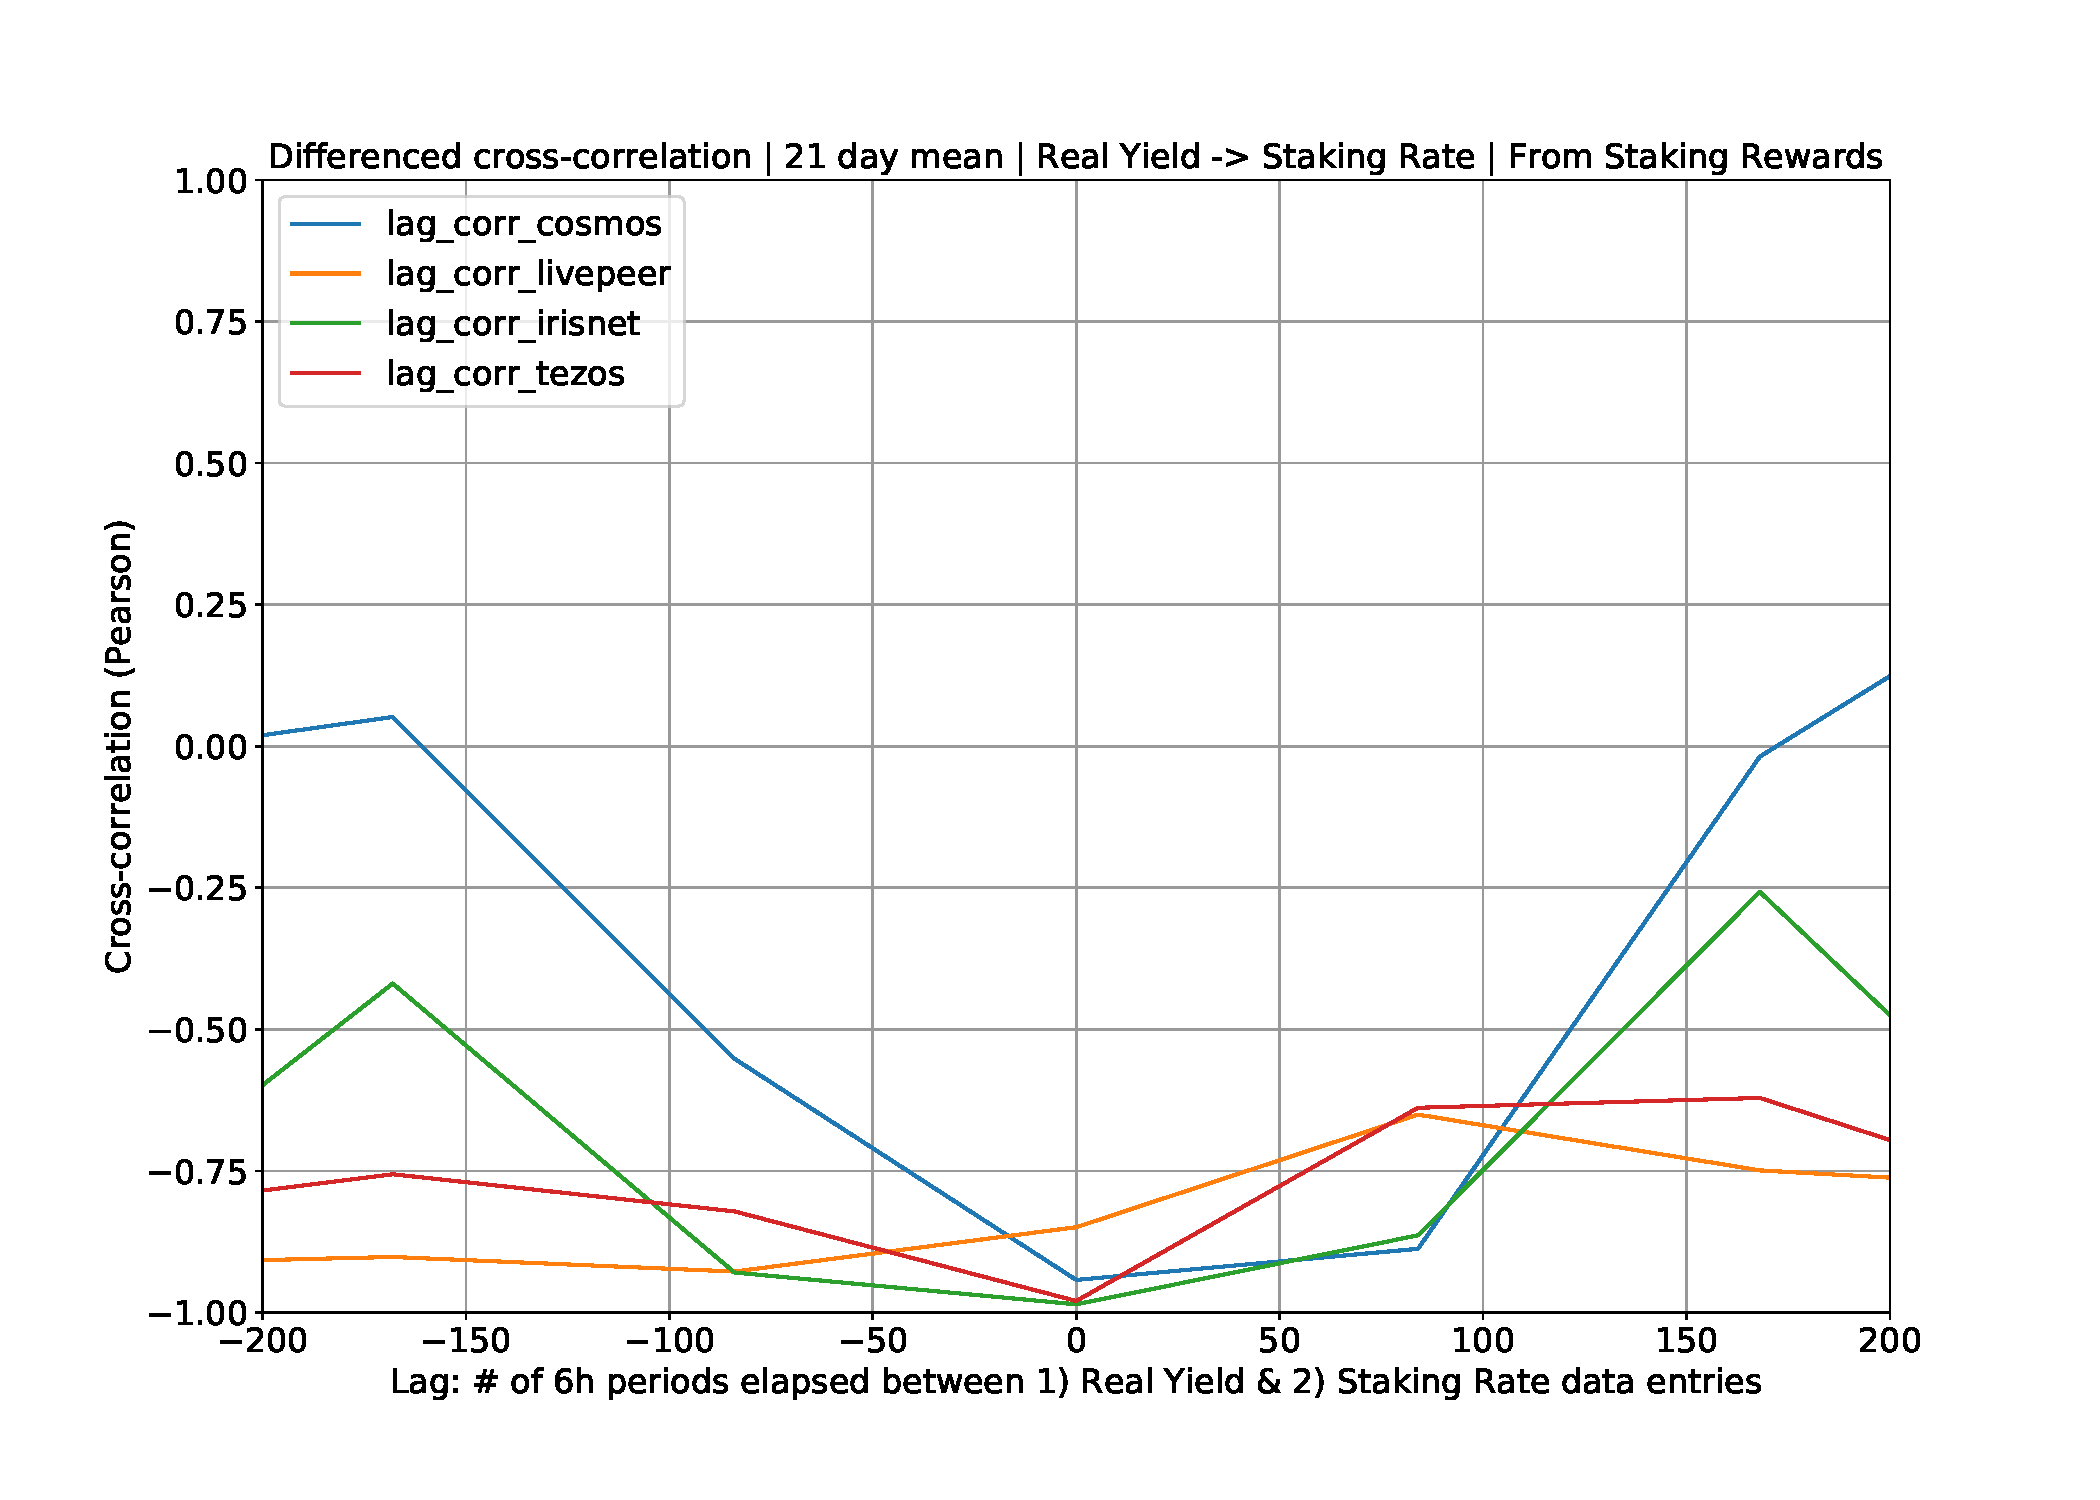
\includegraphics[width=1\textwidth]{graphs/CrossCorr_SR_DIF_21.pdf}
        \caption{21 day lump}
    \end{minipage}\hfill
    \begin{minipage}{0.5\textwidth}
        \centering
        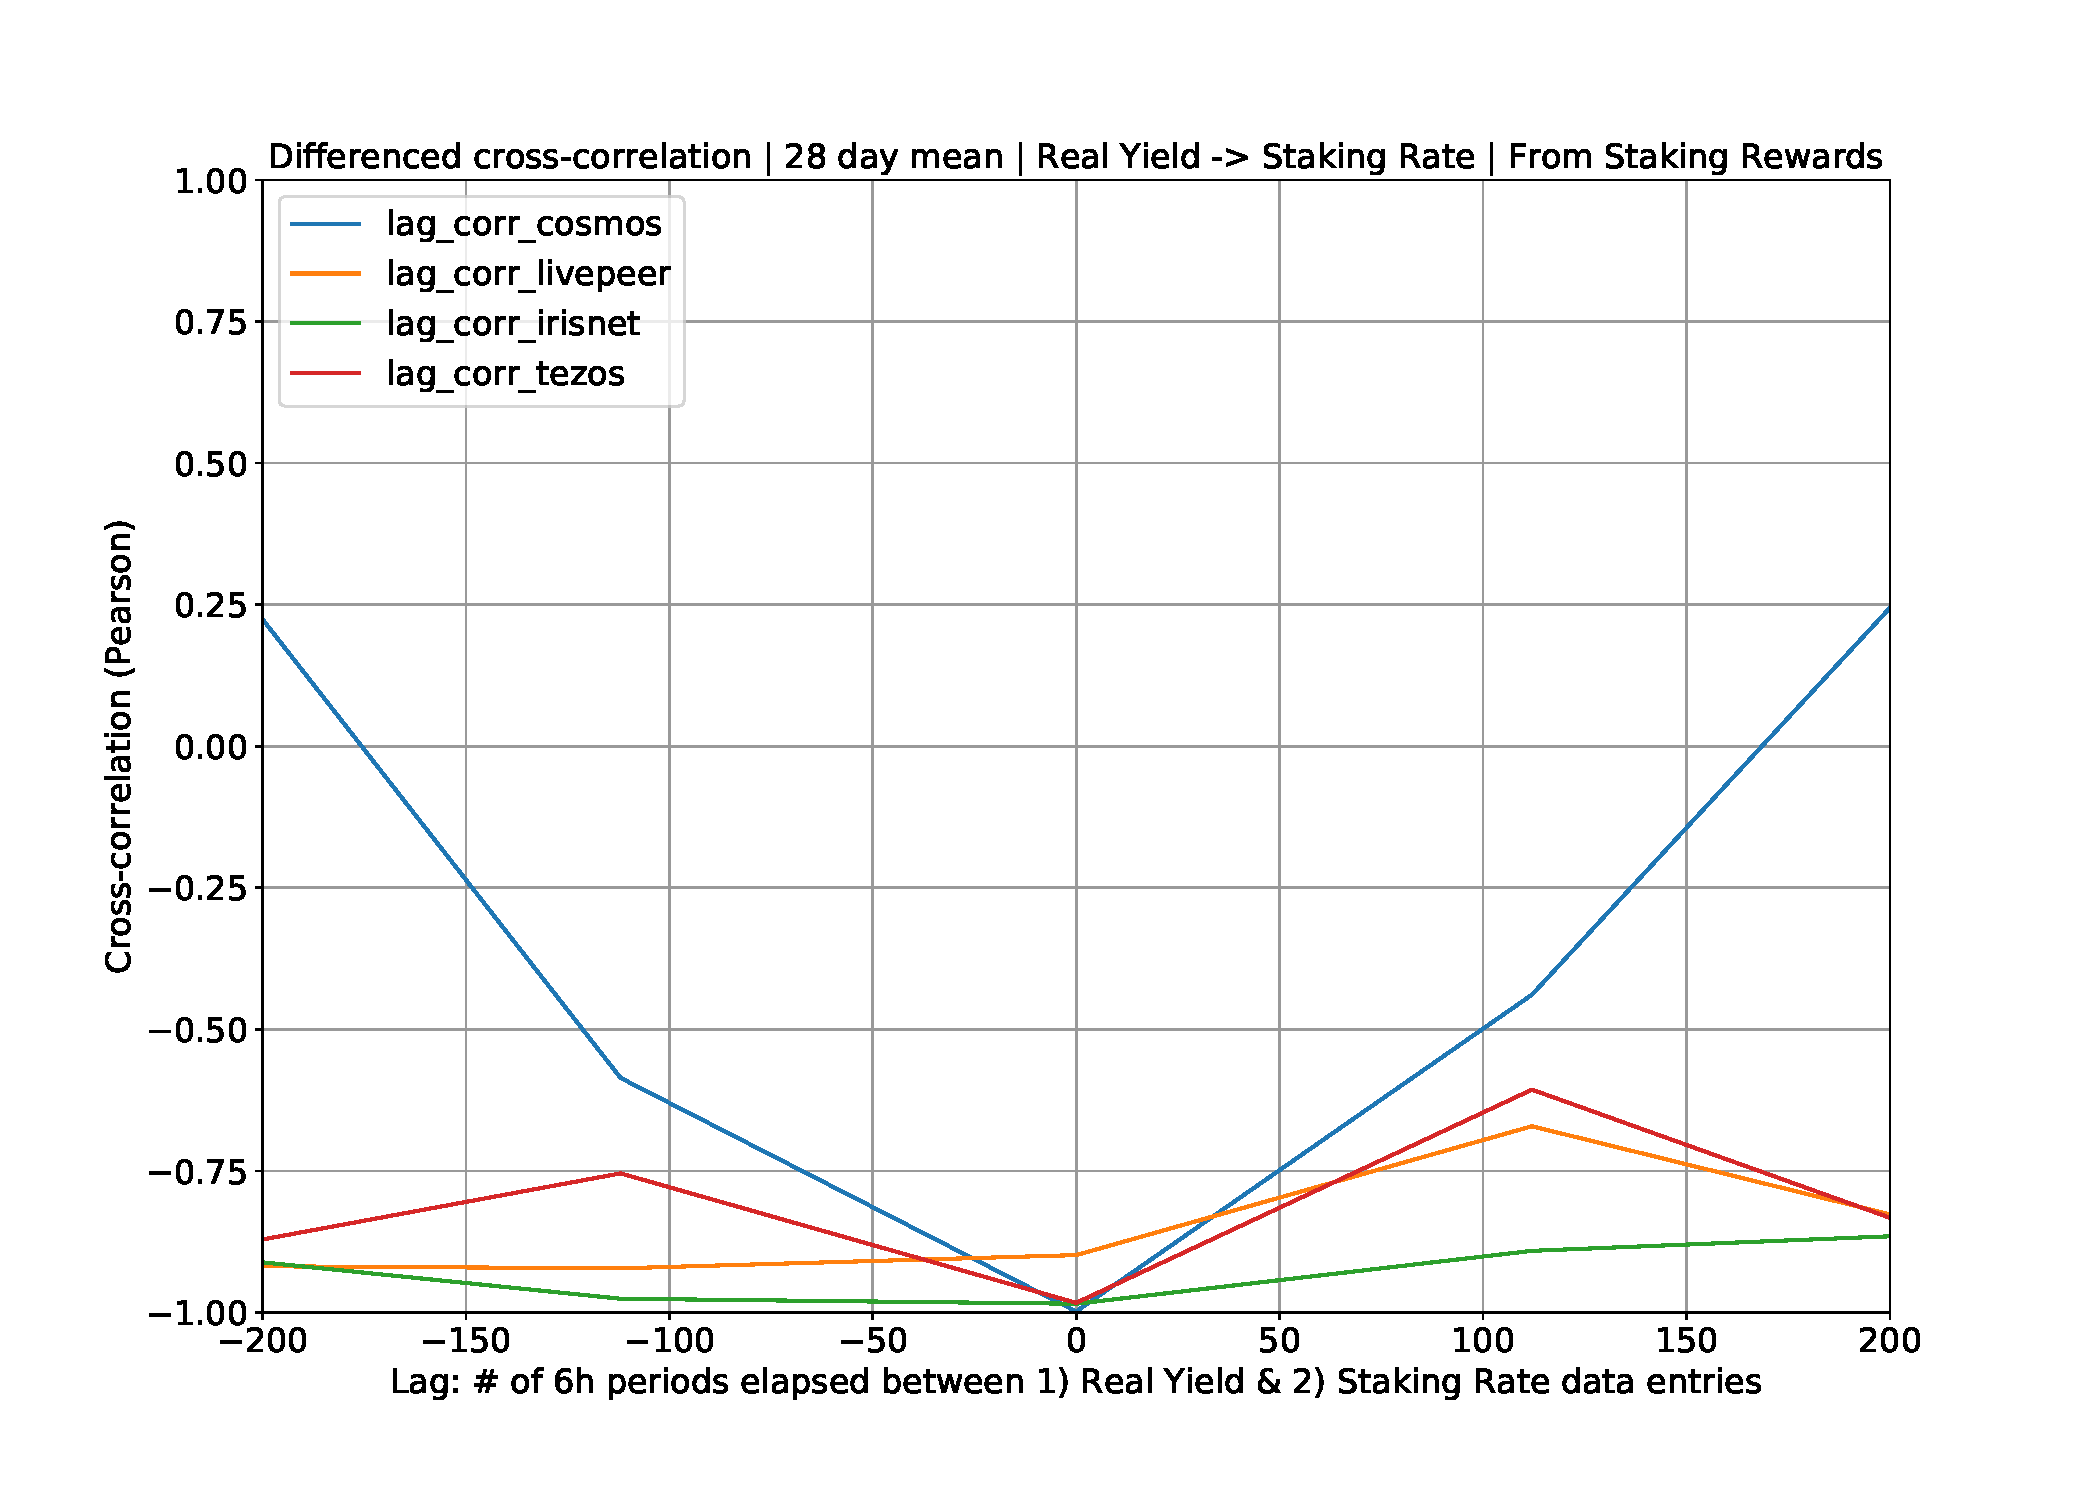
\includegraphics[width=1\textwidth]{graphs/CrossCorr_SR_DIF_28.pdf}
        \caption{28 day lump}
    \end{minipage}
    \caption{Cross-correlation of Real Yield and Staking rate, with a lag of $\pm50$ days instituted between the time series. Each graph shows a different lump size. Note that x-axis is expressed in 6h periods so 200 is equivalent to 50 days. Data from Staking Rewards. N: [Tezos:  1371, Cosmos: 1009, Livepeer: 1148, Irisnet: 1015]}
\end{figure}

\begin{figure}
 \centering
    \begin{minipage}{0.5\textwidth}
        \centering
        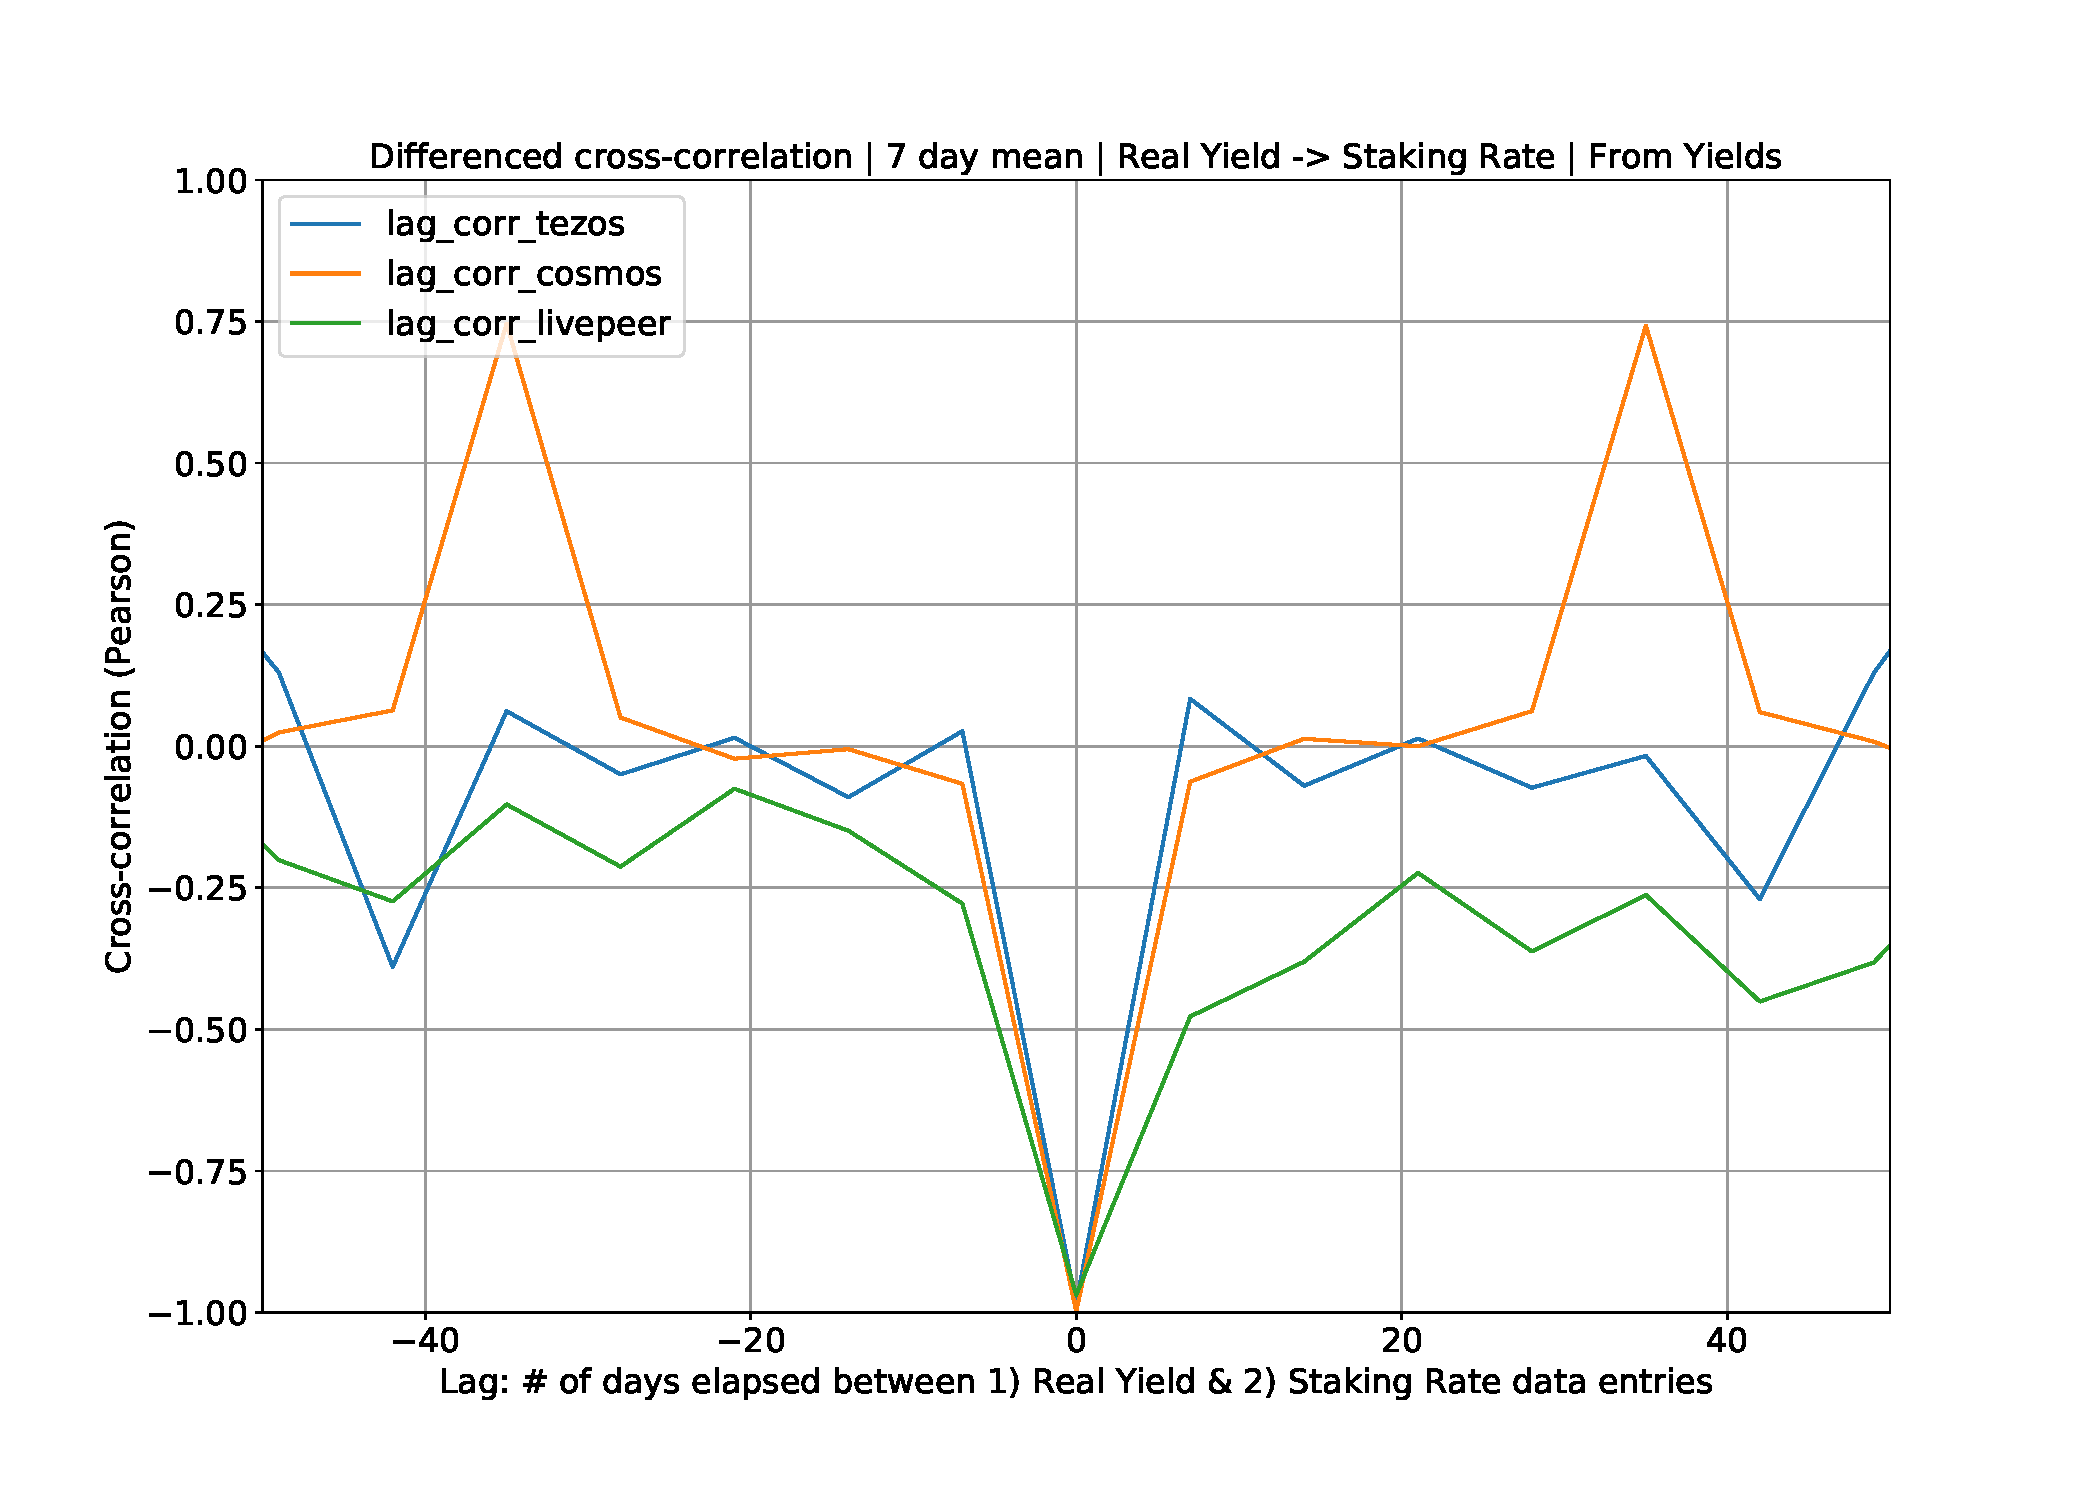
\includegraphics[width=1\textwidth]{graphs/CrossCorr_Yields_DIF_7.pdf}
        \caption{7 day lump}
    \end{minipage}\hfill
    \begin{minipage}{0.5\textwidth}
        \centering
        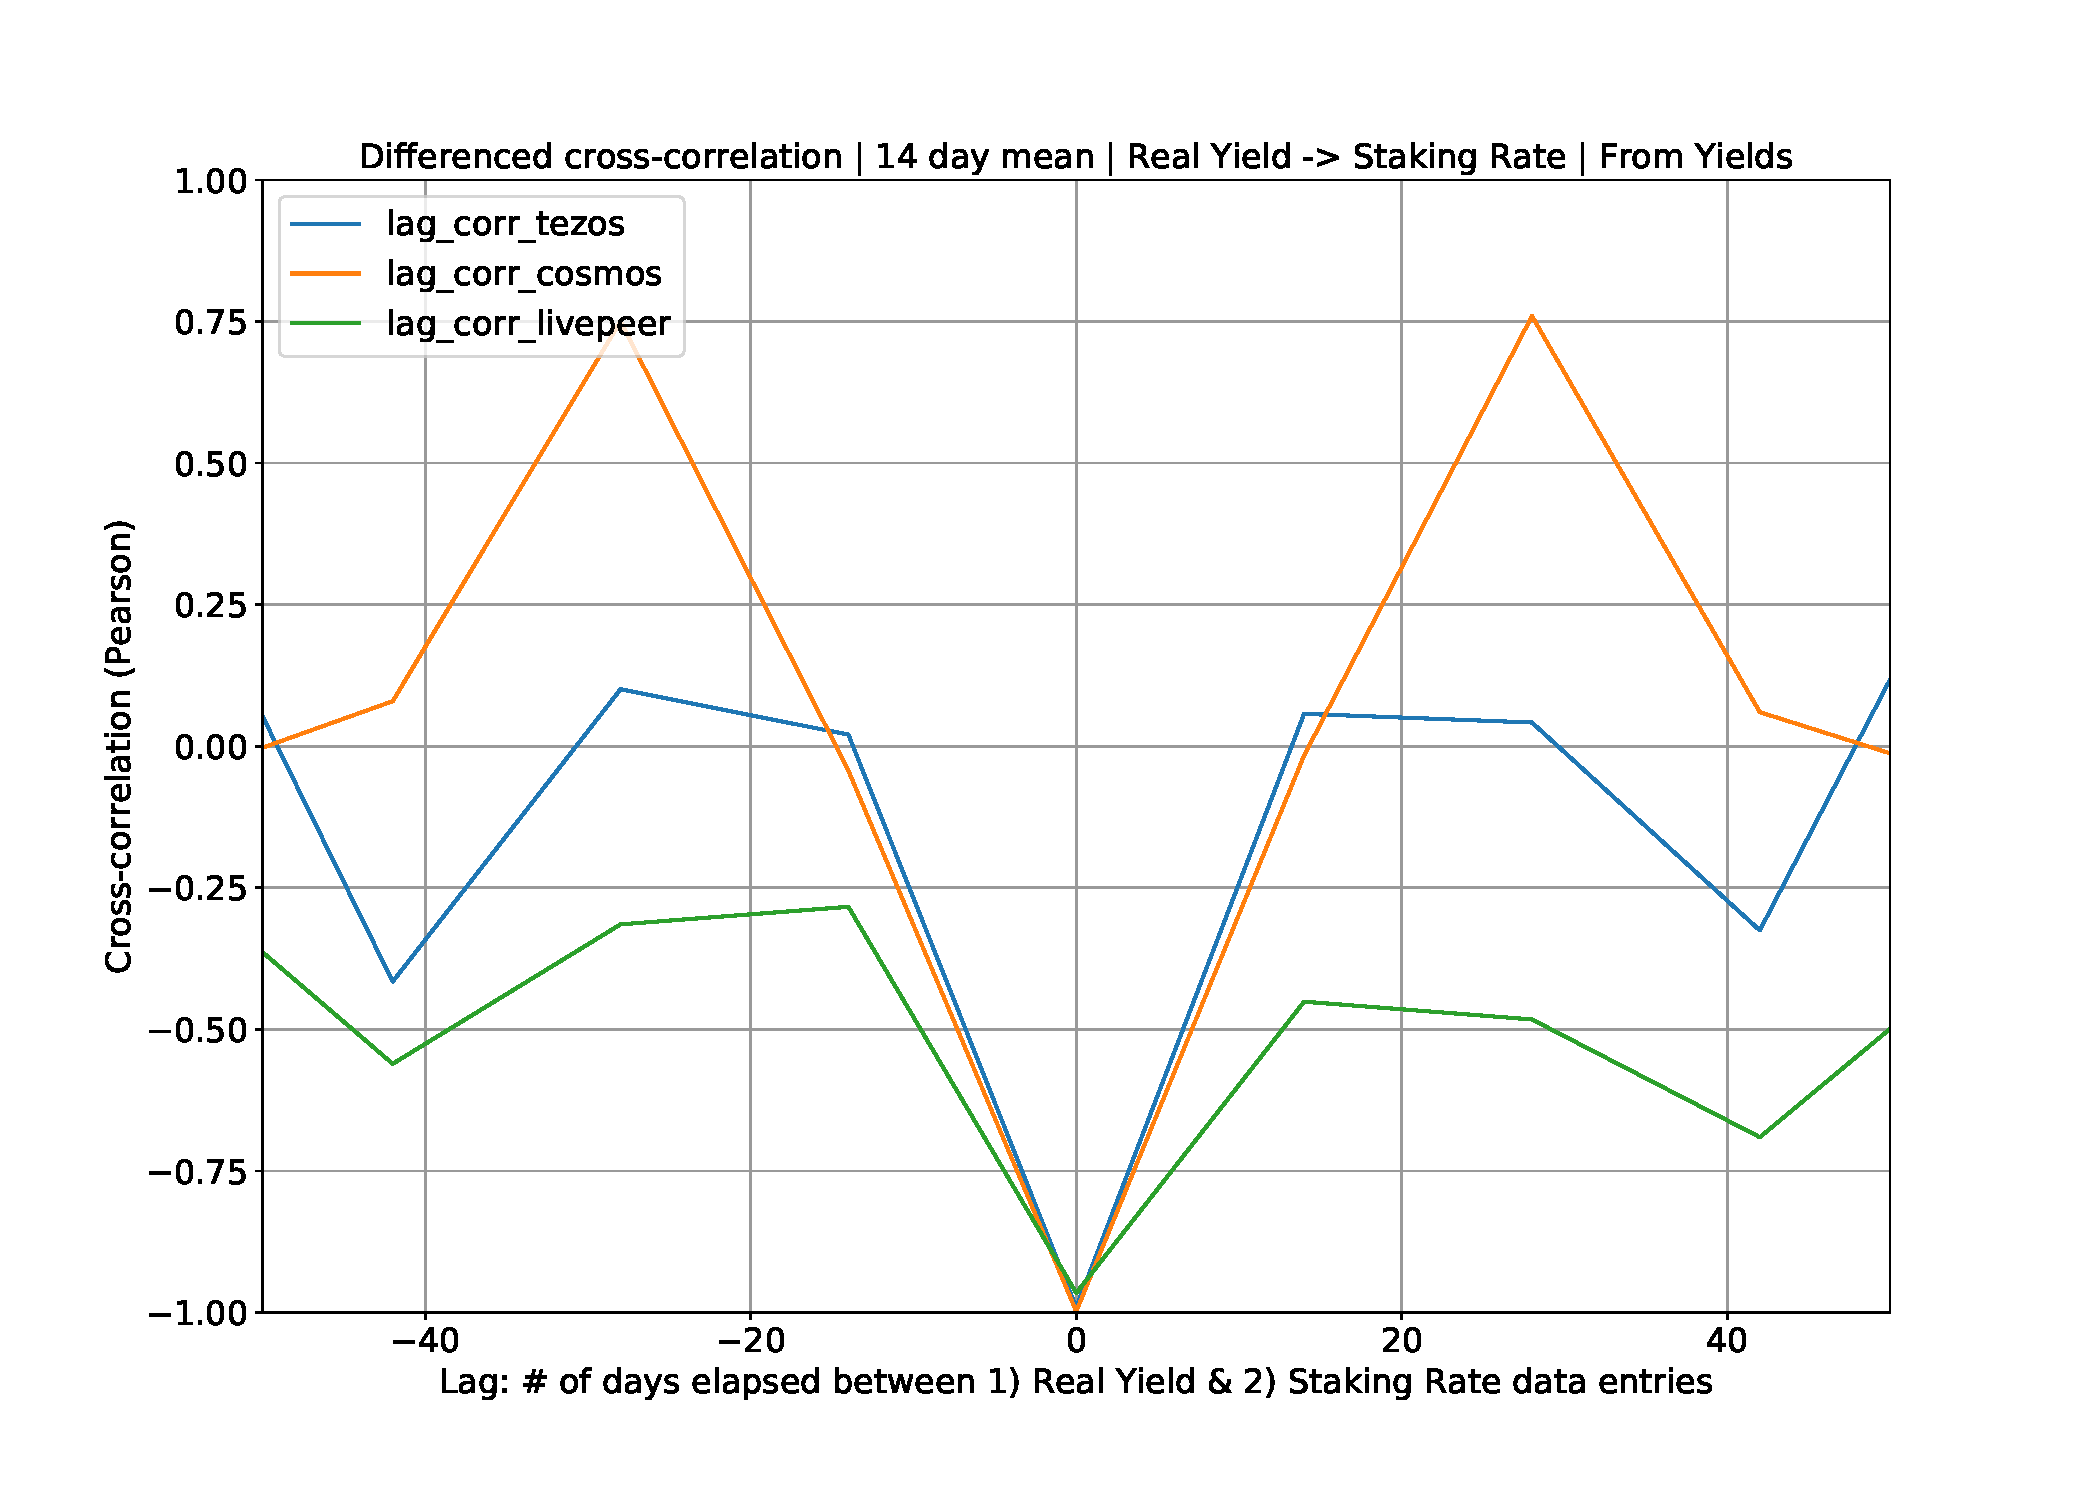
\includegraphics[width=1\textwidth]{graphs/CrossCorr_Yields_DIF_14.pdf}
        \caption{14 day lump}
    \end{minipage}
    \begin{minipage}{0.5\textwidth}
        \centering
        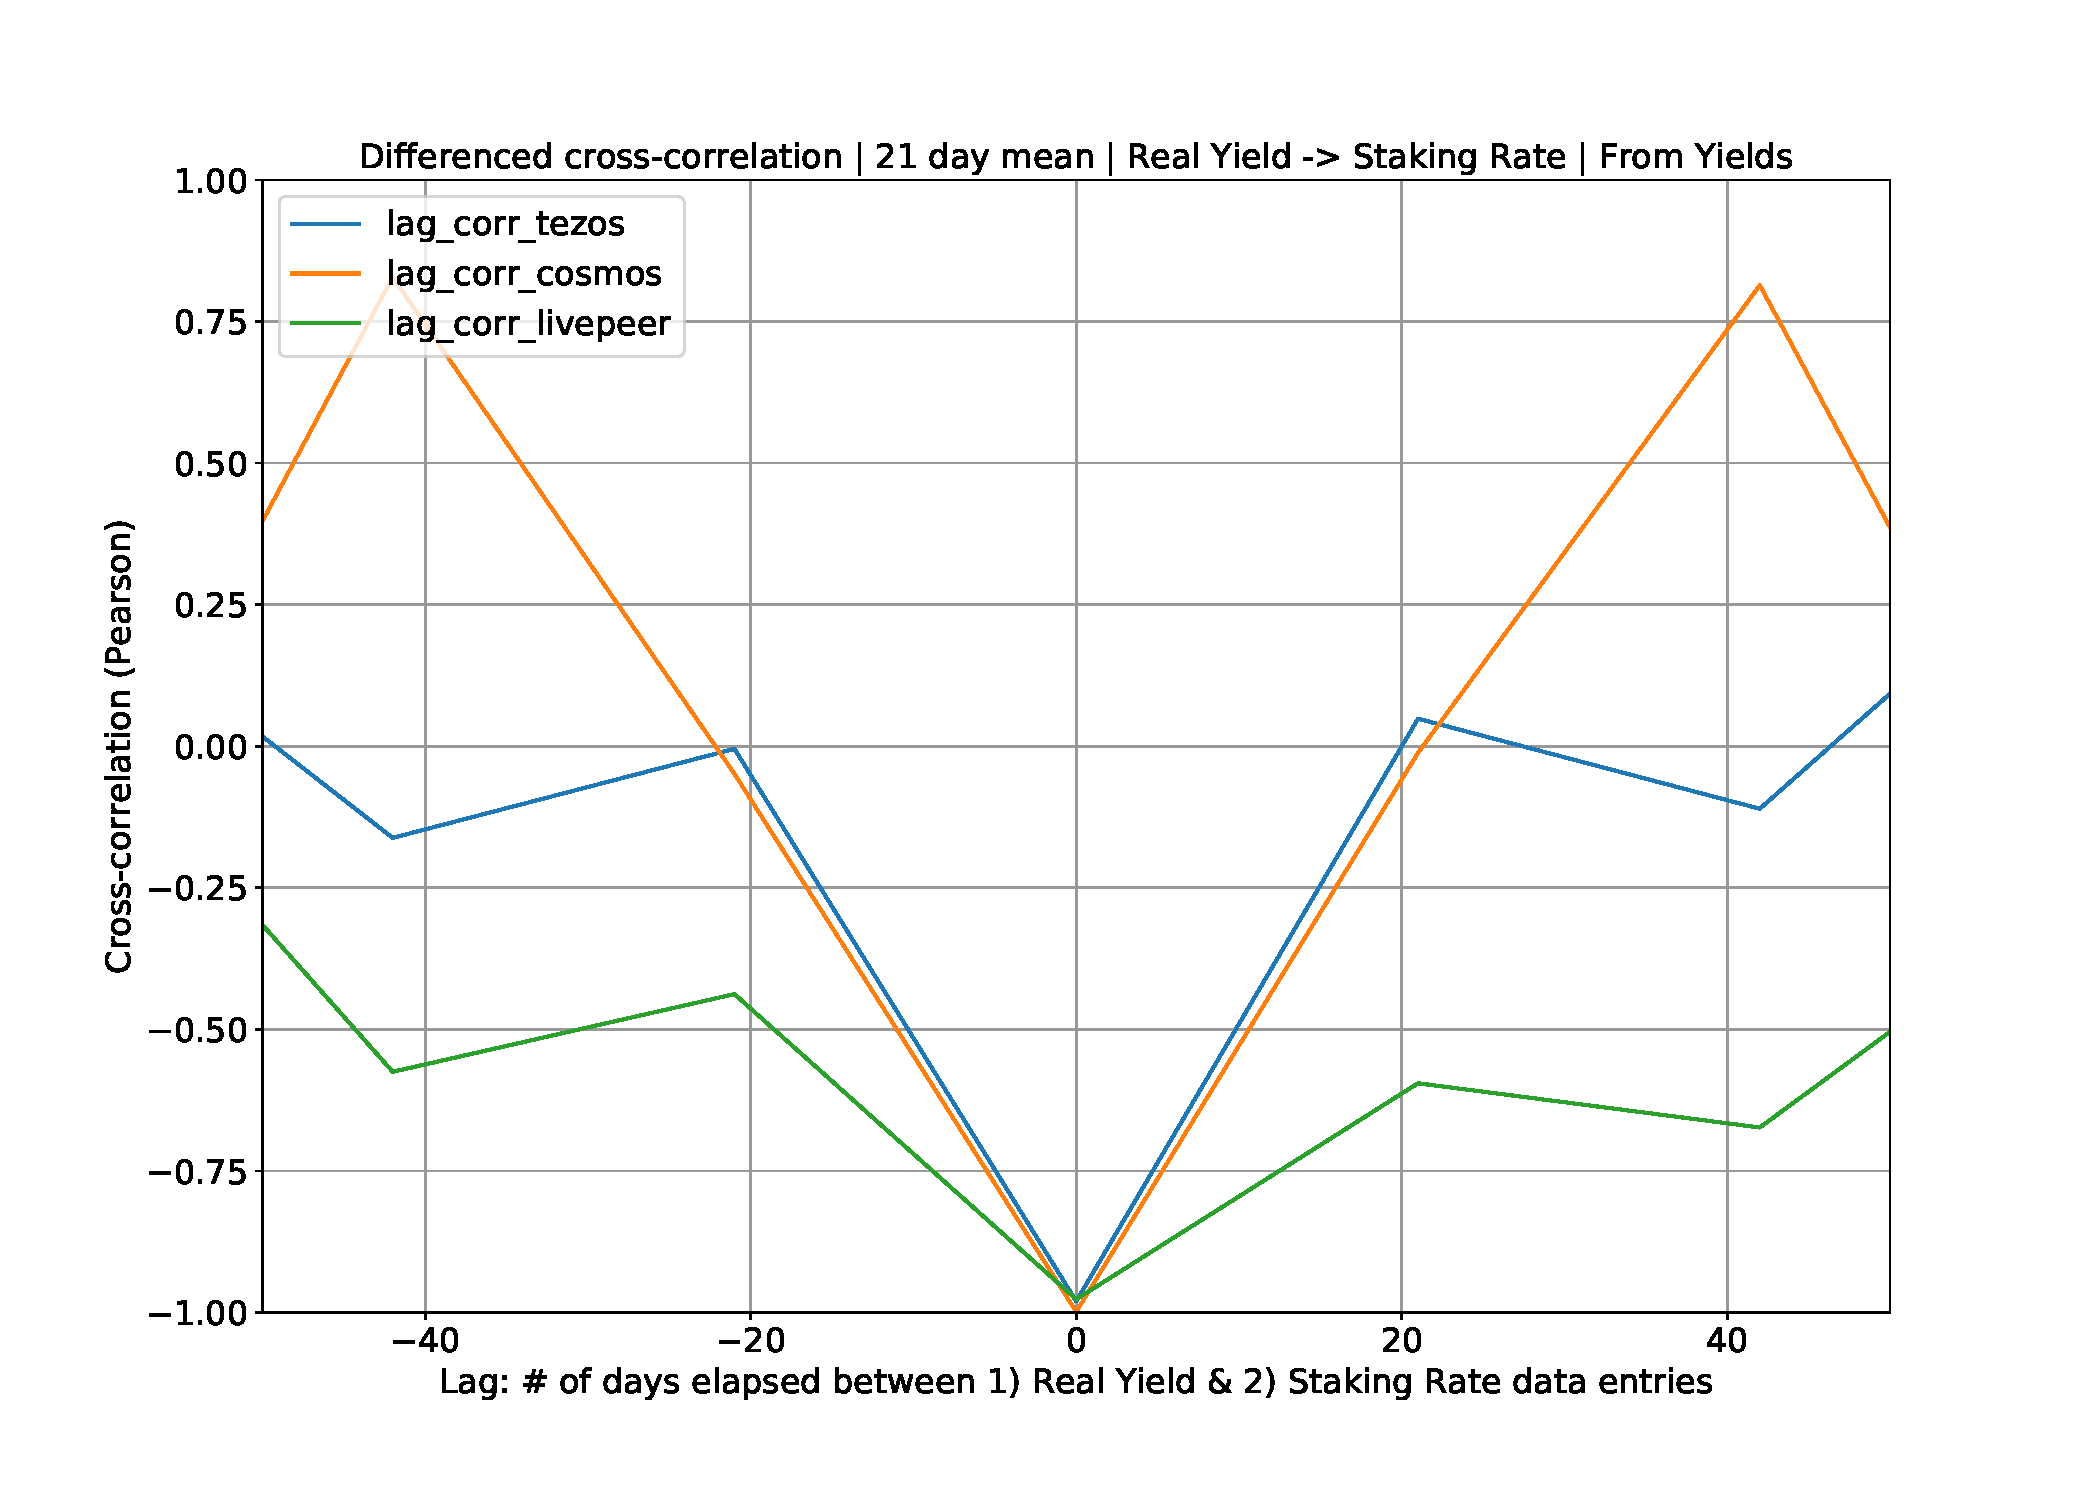
\includegraphics[width=1\textwidth]{graphs/CrossCorr_Yields_DIF_21.pdf}
        \caption{21 day lump}
    \end{minipage}\hfill
    \begin{minipage}{0.5\textwidth}
        \centering
        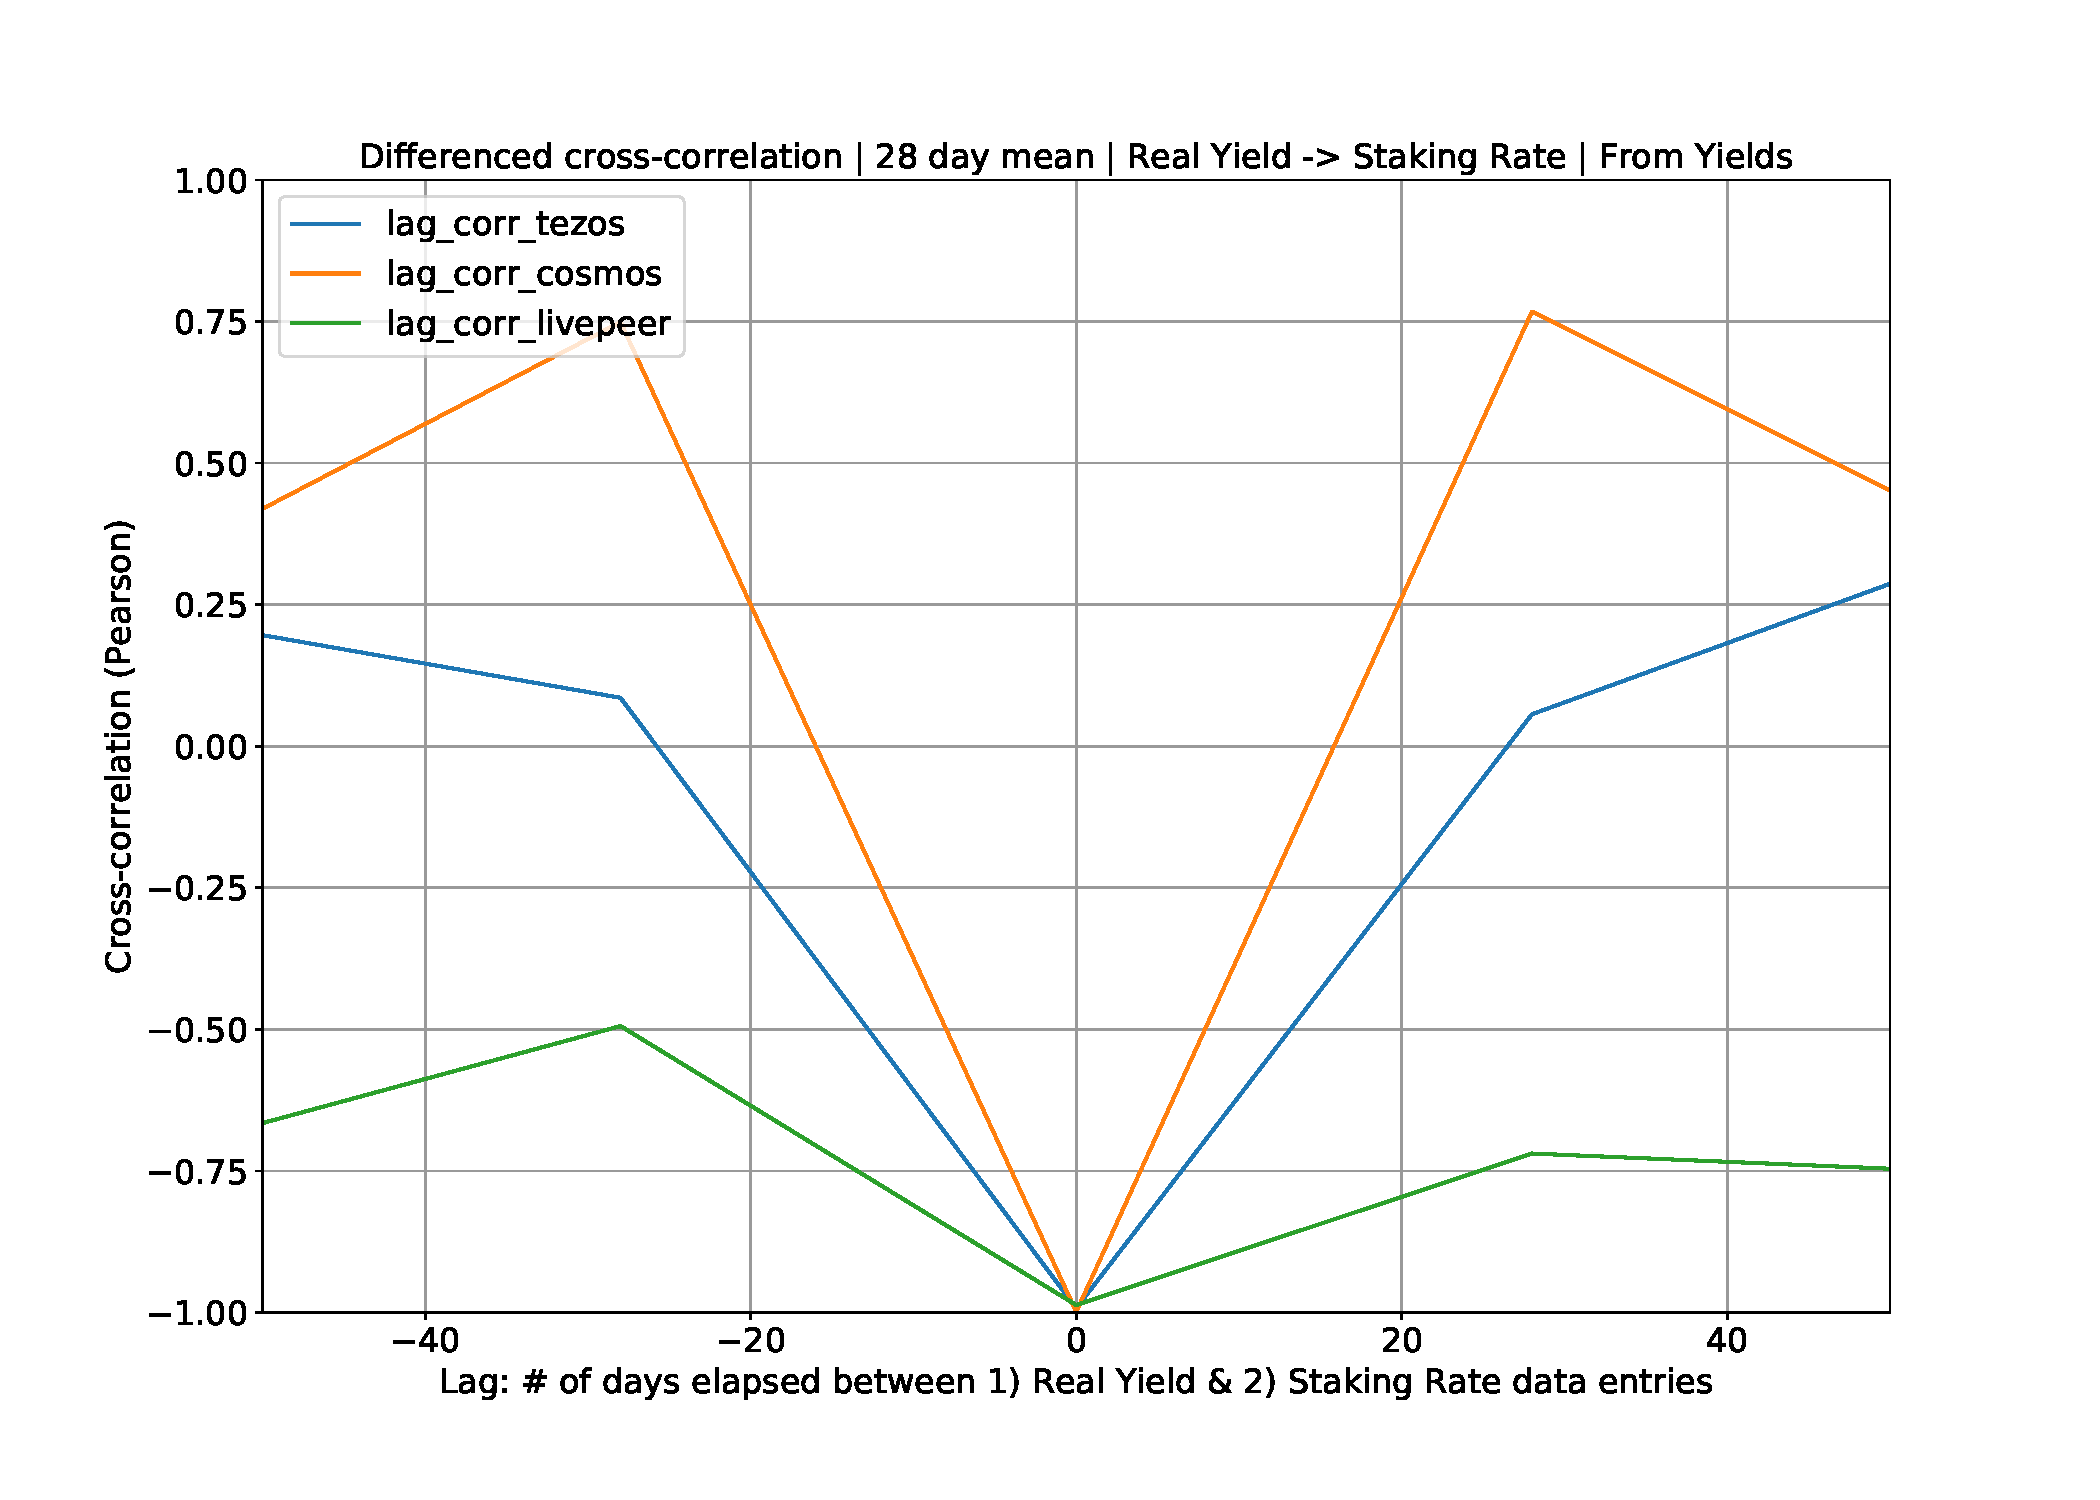
\includegraphics[width=1\textwidth]{graphs/CrossCorr_Yields_DIF_28.pdf}
        \caption{28 day lump}
    \end{minipage}
    \caption{Cross-correlation of Real Yield and Staking rate, with a lag of $\pm50$ days instituted between the time series. Each graph shows a different lump size. Data from Yields. N: [Tezos: 196, Cosmos: 189, Livepeer: 206]}
\end{figure}

\subsubsection{Analysis}

As expected, the cross-correlation is very close to -1 when the lag is zero. This is the manifestation of the known dynamic mentioned in the previous section, where changes in the staking rate immediately impact the real yield. We are interested in the reverse relationship – answering the question; `Does a preceding change in the real yield predict a change in the staking rate?'. This depends on human decision-making and behavior, and occurs over an unknown time lag, if at all. The right hand side of each graph (where the x-axis is positive) shows the results when the real yield data have been shifted, and so real yield readings occur `before' staking rate readings. This is where to look for evidence that the real yield might predict or cause the staking rate.
\\\\
It is notable that the cross-correlations in FIG. (6), FIG. (7), FIG. (8), and FIG. (9) are largely negative or too weak to be conclusive. Indeed, there are no significant positive cross-correlations in any of the Staking Rewards results. In general, the smaller the lag, the stronger the negative correlation. In terms of network, Tezos and Livepeer display the strongest negative correlations. When the data is lumped using the 21 and 28 day means, the networks besides Cosmos produce consistent negative cross-correlations across all lags.
\\\\
The Yields data, shown in FIG. (11), FIG. (12), FIG. (13), and FIG. (14), do not have much in the way of strong cross-correlations, positive or negative, though there is a weak tendency towards the latter. The only exceptions are when the data is lumped using the 21 and 28 day means: Livepeer has strong negative cross-correlations across multiple lags, and Cosmos has a positive cross-correlation at a lag of around 30-40 days. 
\\\\
These results challenge established ideas about staker behavior – a widely-held assumption in staking protocol design is that lower earnings prompt stakers to reduce their stake size, eventually increasing the average earnings for the remaining stakers in the following subsidy rounds, thereby balancing the subsidy mechanism. In other words, protocol designers expect a causal relationship that mirrors the known dynamic (staking rate changing real yield), but perhaps at a slower pace. For this to be possible, we would at the very least need to see positive correlations between the real yield and staking rate once a lag is instituted. We can be agnostic about the magnitude of the lag, but even after 50 days, there is scant evidence that this balancing effect is happening in practice.
\\\\
The second implication of these results is that, in some cases, changes in the real yield appear to prompt the opposite behavior as would be expected. The Staking Rewards data in particular suggests that the collective staker reaction to lower real yields may be to increase their stake. In fact, the negative cross-correlations contain within them two separate `reactions': (1) staking more in response to a lower real yield, and (2) staking less in response to a higher real yield. Crucially, the latter necessarily occurs with a time delay of varying length, depending on the network in question, whereas the former does not. It is not easy to disentangle these two dynamics within the results data. Nevertheless, we can make claims about specific data points – for example, the cross-correlation of -0.965 calculated for Cosmos in FIG. (7). Given that Cosmos's unbonding delay is 21 days, we can attribute this result to stakers depositing more tokens 14 days after lower real yields, as opposed to withdrawing tokens 14 days after higher real yields.
\\\\
More generally, a major unknown in these systems is the staker `reaction time'. One staker could respond to a changing real yield immediately, while another might wait weeks to see if this day-to-day change to evolves into a longer-term trend. Forming conclusions with a single lump size would introduce unacceptable experimenter bias into the results. Of course, 7, 14, 21, and 28 day lumps are not the full story, but they are a decent starting point. Lumps lower than 7 days seem unrealistic, since anecdotally, stakers are not known to change their stake size in response to hourly or daily changes to subsidies. The very weak correlations at the 7 day lump size, relative to longer lumps, go some way in corroborating this. Lumps far greater than 28 days run into sample size issues, where the total number of data points to run a Pearson correlation over drops into the single digits.

\subsubsection{Interpretation with respect to two-phase model}

The fundamental purpose of a subsidies in a decentralized network is to ensure the health and stability of service provision, such that users may be attracted and retained. Subsidy mechanisms are therefore predicated on the notion that service-providers will abandon the network unless they are adequately compensated. The results of this study suggest that, in the early years of a network's existence, this notion is empirically unsubstantiated. None of the networks under examination, based on data from two independent sources, have experienced a shortfall of service-providers, nor are there any observable trends in which decreasing earnings correlate with an increasing paucity of service provision. On the contrary, service-provider sensitivity to decreasing revenue is minimal, or their response involves greater commitment to the network. 
\\\\
One might attribute this ostensibly unshakeable loyalty to a prevalence of long-term strategies, deep pockets, sunk costs, ideological commitment, or even irrational enthusiasm. Some service-providers may respond to lower earnings by staking more because they wish to increase their individual revenue – despite the fact this action will reliably lower everyone's earnings per staked token, including theirs. Regardless of which of these underlying explanations one favours, it is reasonable to conclude that reserving the highest subsidies for the early years of the network is wholly unnecessary. The essence of the two-phase model is maintaining the sum of tokens to be minted over the network's lifetime, but flattening the minting schedule. Therefore the riskiest epoch of the two-phase model, relative to a generic model (i.e. where the issuance falls continuously), is the first few years – where all things equal, the issuance is lower than it would have been. The results demonstrate that, whether due to enthusiasm or deep pockets, service-providers are very unlikely to abandon the network early on. Given the over-arching objective of abundant and reliable service provision, this conclusion derisks the two-phase model.

\bibliography{staking_protocol}

\end{document}
